% ====================================================================
% PLANTILLA INFORME PRIMERA ENTREGA - GEOINFORMÁTICA USACH
% Autor: Prof. Francisco Parra O.
% Archivo Principal (con includes a secciones)
% ====================================================================

\documentclass[11pt,letterpaper]{article}

% PAQUETES ESENCIALES
\usepackage[utf8]{inputenc}
\usepackage[spanish,es-tabla]{babel}
\usepackage[left=2.5cm,right=2.5cm,top=2.5cm,bottom=2.5cm]{geometry}
\usepackage{graphicx}
\usepackage{float}
\usepackage{xcolor}
\usepackage{hyperref}
\usepackage{amsmath,amssymb}
\usepackage{booktabs}
\usepackage{caption}
\usepackage{newunicodechar}
\newunicodechar{≥}{\geq}
\usepackage{subcaption}
\usepackage{longtable}
\usepackage{array}
\usepackage{multirow}
\usepackage{listings}
\usepackage{fancyhdr}
\usepackage{lastpage}
\usepackage[backend=biber,style=apa]{biblatex}

% Configuración de bibliografía
%\addbibresource{referencias.bib} % Crear este archivo para las referencias

% Colores institucionales
\definecolor{usachblue}{RGB}{0,46,93}
\definecolor{usachred}{RGB}{200,16,46}
\definecolor{codegreen}{rgb}{0,0.6,0}
\definecolor{codegray}{rgb}{0.5,0.5,0.5}
\definecolor{codepurple}{rgb}{0.58,0,0.82}
\definecolor{backcolour}{rgb}{0.95,0.95,0.92}

% Configuración de código
\lstdefinestyle{mystyle}{
    backgroundcolor=\color{backcolour},
    commentstyle=\color{codegreen},
    keywordstyle=\color{magenta},
    numberstyle=\tiny\color{codegray},
    stringstyle=\color{codepurple},
    basicstyle=\ttfamily\footnotesize,
    breakatwhitespace=false,
    breaklines=true,
    captionpos=b,
    keepspaces=true,
    numbers=left,
    numbersep=5pt,
    showspaces=false,
    showstringspaces=false,
    showtabs=false,
    tabsize=2,
    language=Python
}
\lstset{style=mystyle}

% Configuración de hyperref
\hypersetup{
    colorlinks=true,
    linkcolor=usachblue,
    filecolor=magenta,
    urlcolor=usachblue,
    citecolor=usachblue
}

% Encabezado y pie de página
\pagestyle{fancy}
\fancyhf{}
\lhead{\textcolor{usachblue}{Geoinformática - Primera Entrega}}
\rhead{\textcolor{usachblue}{USACH 2025}}
\lfoot{\small\textit{Terramatch}}
\cfoot{\thepage\ de \pageref{LastPage}}
\rfoot{\today}

% ====================================================================
% INICIO DEL DOCUMENTO
% ====================================================================

\begin{document}

% Portada
% ====================================================================
% PORTADA - MODIFICAR CON SUS DATOS
% ====================================================================

\begin{titlepage}
    \centering
    \vspace*{1cm}

    \Large{\textbf{UNIVERSIDAD DE SANTIAGO DE CHILE}}\\
    \large{Facultad de Ingeniería}\\
    \large{Departamento de Ingeniería Informática}\\

    \vspace{3cm}

    \rule{\textwidth}{0.5mm}\\
    \vspace{0.5cm}

    {\LARGE\textbf{TerraMatch}}\\
    \vspace{0.3cm}
    {\Large\textit{Sistema de estimación de satisfacción inmobiliaria basado en información geoespacial}}\\

    \vspace{0.5cm}
    \rule{\textwidth}{0.5mm}

    \vspace{2cm}

    {\Large\textbf{Primera Evaluación}}\\
    \vspace{0.5cm}
    {\large Informe de Avance}

    \vspace{3cm}

\begin{minipage}{0.8\textwidth}
    \begin{flushleft}
        \large
        \textbf{Integrantes del Grupo:}\\
        Valentina Del Pilar Barr\'ia - 21.149.435-2\\
        Felipe Baeza Mu\~noz - 20.637.464-0\\
        Byron Caices Lima - 20.915.795-0\\
        Catalina L\'opez - 21.051.116-4\\
        Jaime Antonio Riquelme Olguin - 20.964.708-7\\
        Diego Ignacio Rojas Bustos - 17.464.162-5\\
        \vspace{0.5cm}
        \textbf{Profesor:}\\
        Francisco Parra O.\\
        \vspace{0.5cm}
        \textbf{Ayudantes:}\\
        %[Si aplica]
    \end{flushleft}
\end{minipage}


    \vfill

    {\large \today}
\end{titlepage}


% Resumen Ejecutivo
% ====================================================================
% RESUMEN EJECUTIVO
% ====================================================================

\newpage
\section*{Resumen Ejecutivo}
\addcontentsline{toc}{section}{Resumen Ejecutivo}

% [Máximo 1 página]
% Incluir: problema abordado, área de estudio, metodología principal,
% resultados preliminares clave, y próximos pasos.

El mercado inmobiliario chileno atraviesa una crisis de acceso a la vivienda caracterizada por el requisito de un 20\% de pie inicial para créditos hipotecarios, monto que representa aproximadamente 32 veces el ingreso mediano del país y que coloca a numerosos hogares en una situación donde no califican para créditos bancarios ni para subsidios estatales. Esta realidad ha generado consumidores cada vez más exigentes que buscan maximizar la satisfacción de su inversión inmobiliaria, demandando herramientas objetivas que les permitan evaluar propiedades más allá del precio. En este contexto, TerraMatch surge como un sistema de apoyo a la decisión que integra información geoespacial para estimar la satisfacción residencial potencial de propiedades en venta.

El proyecto se desarrolla sobre cuatro comunas de la Región Metropolitana de Santiago: Estación Central, La Reina, Ñuñoa y Santiago Centro. Esta selección responde a criterios de diversidad socioeconómica (desde estratos altos en La Reina hasta medios-bajos en Estación Central), heterogeneidad urbana (zonas de alta densificación vertical versus sectores residenciales tradicionales) y disponibilidad de datos suficientes para el entrenamiento de modelos predictivos.

La metodología implementada comprende cinco etapas: extracción automatizada de 7.702 propiedades mediante web scraping de Portal Inmobiliario, geocodificación de direcciones utilizando Google Maps API en el sistema de coordenadas EPSG:32719 (UTM Zone 19S), cálculo de 42 variables espaciales mediante distancias euclidianas a puntos de interés (estaciones de metro, centros educacionales, de salud, seguridad, comercio y áreas verdes), diseño de un índice de satisfacción residencial como variable objetivo, y entrenamiento de modelos predictivos mediante Machine Learning.

Los resultados preliminares demuestran que el modelo exploratorio híbrido GWRF por cluster explica el 88\% de la varianza observada con un error medio absoluto de 439 UF/m². Tras una comparación exhaustiva de algoritmos, el modelo LightGBM fue seleccionado como modelo final, alcanzando un R² de 0.8635 con RMSE de 0.3357 y baja autocorrelación espacial de residuos (Moran's I = 0.0695), lo que indica ausencia de sesgo geográfico en las predicciones. Las próximas fases contemplan la expansión geográfica a comunas adicionales, incorporación de variables temporales, desarrollo de API REST para predicciones en tiempo real, implementación de interfaz web interactiva, y validación mediante encuestas de satisfacción real de usuarios.


% Índice
\newpage
\tableofcontents
\newpage

% Sección 1: Introducción
% ====================================================================
% INTRODUCCIÓN
% ====================================================================

\section{Introducción}

\subsection{Contexto y Motivación}

% Explicar el contexto del problema, por qué es importante,
% y qué motivó la selección de este proyecto
Entre 2021 y 2023 comenzo una fuerte contracción en la demanda de viviendas, especialmente en el segmento de casas nuevas sin subsidio que cayó un 11,8\% entre enero y octubre de 2023, las ventas de casas nuevas alcanzaron en octubre de este año a tan solo 330 unidades con una tasa de desistimientos del 33\% en casas sin subsidio y del 15\% en departamentos, niveles históricamente altos a esta alturas del año. Este desplome se debio al deterioro de las condiciones de crédito, el aumento de las tasas de interés, restricciones bancarias y el impacto de la inflación sobre la capacidad de endeudamiento manteniendose durante los años siguientes.
\\ 
Debido a lo anterior a comienzos del 2025 el alto stock de propiedades no vendidas, estimado en alrededor de 70.000 unidades, comenzo a transformar el mercado inmobiliario ofreciendo unas nueva posibilidades para compradores que buscan oportunidades de inversión o vivienda propia, especialmente mediante ofertas directas o grupos de compra \cite{biobio_ciper_2025}.
\\Segun el estudio ``monitor de viviendas 2025'' \cite{ipsos_monitor_2025} realizado por la consultora multinacional IPSOS en enero de este año 2025 mostro que el "60 \% de los encuestados estan contentos con la situacion actual de la vivienda" en Chile, de donde "tres de cada cuatro (74\%) propietarios esta satisfecho con su situacion de vivienda" y "solo cuatro de diez arrendatarios (39\%) dice estar feliz de su situacion habitacional", lo que alienta a nuevos clientes y a actuales arrendatarios a considerar la inversion inmobiliaria como un objetivo plausible en el actual contexto chileno.
\\
\\Respecto a esto se ha determinado que los principales desafios para los clientes al momento de comprar o arrendar una vivienda se identifican de la siguiente forma:

\begin{itemize}
    \item Precios altos de la propiedades
    \item Tasas de interes muy altas
    \item Aumento de los costos de construccion de viviendas y edificios
\end{itemize}
Esta dificultad para conseguir vivienda a llevado a que los clientes tomen en consideracion los siguientes aspectos al momentos de comprar una propiedad:

\begin{itemize}
    \item Relación precio-m²
    \item Tasa de delincuencia
    \item Ubicacion y servicios
    \item Acceso al transporte publico
    \item Espacio al aire libre
    \item Privacidad
    \item Buena infraestructura local
\end{itemize}

Por todo lo anterior, hoy se presenta una oportunidad interesante dentro del mundo inmobiliario chileno: la capacidad de influir en las decisiones de potenciales clientes para informar y convencer al cliente indeciso de comprar una vivienda con datos geoespaciales que le ayuden a determinar una opción de vivienda que satisfaga sus necesidades a un precio asequible.

\subsection{Objetivos}

\subsubsection{Objetivo General}

% Un objetivo general claro y alcanzable
Desarrollar un sistema de recomendación inmobiliaria inteligente que prediga la satisfacción residencial de propiedades en venta mediante la integración de características internas de las viviendas con factores geoespaciales del entorno urbano, empleando técnicas de Machine Learning (LightGBM) para proporcionar recomendaciones personalizadas que faciliten la toma de decisiones de compra en el mercado inmobiliario de la Región Metropolitana de Santiago.

\subsubsection{Objetivos Específicos}

\begin{enumerate}
    \item \textbf{Consolidar y normalizar información geoespacial}: Integrar 29 datasets geográficos heterogéneos de la Región Metropolitana, normalizando sistemas de coordenadas al CRS EPSG:32719 (UTM Zone 19S), validando calidad geométrica, y estandarizando estructuras de datos para garantizar consistencia y trazabilidad en el análisis espacial.
    
    \item \textbf{Cuantificar características espaciales del entorno urbano}: Generar una grilla sistemática de evaluación sobre el territorio de estudio y calcular 72 métricas espaciales cuantitativas por ubicación, incluyendo: (a) distancias euclidianas a 21 categorías de servicios urbanos, (b) densidades de servicios en radios de 300m, 600m y 1000m, y (c) índices compuestos de accesibilidad en 9 dimensiones de habitabilidad.
    
    \item \textbf{Recopilar y geocodificar datos del mercado inmobiliario}: Obtener mediante web scraping información de 7,702 propiedades en venta (casas y departamentos) de 4 comunas objetivo (La Reina, Ñuñoa, Santiago Centro, Estación Central), geocodificar direcciones mediante Google Maps API, y validar coherencia entre características de propiedades y ubicaciones geográficas.
    
    \item \textbf{Desarrollar proxy de satisfacción residencial}: Diseñar e implementar un índice de satisfacción (escala 1-10) que integre: (a) valor económico relativo (precio/m² contextualizado), (b) características físicas de la propiedad (espacio, distribución), y (c) accesibilidad a servicios urbanos, con capacidad de personalización mediante 5 perfiles de usuario (familia con niños, profesional joven, inversionista, adulto mayor, balanceado).
    
    \item \textbf{Entrenar y validar modelo predictivo de satisfacción}: Implementar modelo LightGBM para predecir satisfacción residencial utilizando 42 features (características internas + métricas espaciales), alcanzar $R^2 \geq 0.85$ en conjunto de prueba, validar mediante cross-validation 5-fold, analizar importancia de variables, y evaluar autocorrelación espacial de residuos para verificar ausencia de sesgo geográfico.

    \item \textbf{Desarrollar API de recomendación}: Crear sistema de predicción funcional que permita: (a) estimar satisfacción de propiedades nuevas, (b) generar rankings personalizados por perfil de usuario, (c) comparar múltiples opciones simultáneamente, y (d) explicar factores determinantes de cada predicción mediante análisis de importancia de variables.
    \item \textbf{Visualizar patrones espaciales y resultados}: Generar 3 mapas temáticos con elementos cartográficos estándar (ubicación de propiedades, distribución de precios, satisfacción predicha), 5 gráficos estadísticos de análisis exploratorio (histogramas, correlaciones, dispersión, importancia de variables), y 1 visualización interactiva web (mapa Folium con popups informativos y heatmap).
    \item \textbf{Evaluar desempeño comparativo de modelos}: Implementar línea base con Random Forest, comparar rendimiento con al menos 3 algoritmos adicionales (XGBoost, CatBoost, Neural Networks), documentar métricas de evaluación (R², RMSE, MAE, tiempo de entrenamiento), y justificar selección del modelo final mediante análisis cuantitativo de trade-offs precisión-interpretabilidad-eficiencia.
    
\end{enumerate}

\subsection{Preguntas de Investigación}

\
El proyecto busca responder las siguientes preguntas clave mediante análisis geoespacial cuantitativo:

\subsubsection{Pregunta Principal}

\textbf{¿Qué hace que una vivienda sea satisfactoria para vivir en el contexto urbano de Santiago?}

Esta pregunta se descompone en sub-preguntas específicas que el proyecto aborda:

\begin{enumerate}
    \item \textbf{Dimensión económica}: ¿Cuál es la relación entre el valor económico (precio/m²) y la satisfacción percibida? ¿Propiedades más caras son necesariamente más satisfactorias?
    
    \item \textbf{Dimensión espacial}: ¿En qué medida los factores externos (proximidad a servicios, áreas verdes, transporte) determinan la satisfacción residencial más allá de las características internas de la propiedad?
    
    \item \textbf{Heterogeneidad de preferencias}: ¿Cómo varían los determinantes de satisfacción según el perfil del usuario? (familias vs. profesionales jóvenes vs. adultos mayores vs. inversionistas)
\end{enumerate}

\subsubsection{Preguntas Secundarias}

\begin{itemize}
    \item \textbf{Autocorrelación espacial}: ¿Existe dependencia espacial en la satisfacción residencial? Es decir, ¿viviendas cercanas tienden a tener niveles similares de satisfacción debido a características compartidas del entorno?
    
    \item \textbf{Importancia relativa de factores}: ¿Cuáles son las 10 variables más determinantes de satisfacción? ¿Son características internas (superficie, dormitorios) o factores espaciales externos (distancia a metro, áreas verdes)?
    
    \item \textbf{Gradientes urbanos}: ¿Existen patrones geográficos sistemáticos? ¿La satisfacción aumenta/disminuye con la distancia al centro urbano o sigue otros patrones espaciales?
    
    \item \textbf{Equidad territorial}: ¿Qué comunas ofrecen mejor relación calidad-precio? ¿Existen zonas con alta satisfacción predicha pero precios relativamente accesibles?
    
    \item \textbf{Capacidad predictiva}: ¿Es posible predecir con alta precisión (R² > 0.85) la satisfacción residencial utilizando únicamente características observables y datos geográficos públicos?
    
    \item \textbf{Accesibilidad diferenciada}: ¿Qué dimensiones de accesibilidad (transporte, educación, salud, seguridad, áreas verdes) tienen mayor peso en la satisfacción? ¿Este peso varía según el tipo de propiedad (casa vs. departamento)?
\end{itemize}

\subsubsection{Hipótesis de Trabajo}

Basándonos en la literatura de geografía urbana y economía espacial, planteamos:


latex\begin{itemize}
    \item \textbf{H1}: La satisfacción residencial está significativamente influenciada por factores espaciales externos, más allá del precio y características internas de la vivienda.
    
    \item \textbf{H2}: Existe autocorrelación espacial positiva en la satisfacción residencial (Moran's $I > 0$), indicando clustering de zonas de alta/baja satisfacción.
    
    \item \textbf{H3}: La importancia relativa de factores varía sustancialmente entre perfiles de usuario, siendo transporte crítico para profesionales jóvenes, educación para familias, y salud para adultos mayores.
    
    \item \textbf{H4}: Modelos de Machine Learning que integran características espaciales superan en capacidad predictiva ($R^2 > +10\%$) a modelos que solo consideran atributos de la propiedad.
\end{itemize}


\subsection{Alcance y Limitaciones}

\subsubsection{Alcance Geográfico}
Este proyecto considera información geoespacial para las siguientes cuatro comunas de la Región Metropolitana de Santiago:

\begin{itemize}
    \item Ñuñoa
    \item La Reina
    \item Santiago Centro
    \item Estación Central
\end{itemize}

\subsubsection{Datos de Propiedades}
El análisis contempla un total de \textbf{7,702 propiedades} en venta, distribuidas en:
\begin{itemize}
    \item 5,135 departamentos
    \item 2,567 casas
\end{itemize}

Con las siguientes características:
\begin{itemize}
    \item Rango de precios: 800 - 73,000 UF
    \item Superficie: 16 - 900 m²
    \item Fuente: Portal Inmobiliario (web scraping) + Google Maps API (geocodificación)
\end{itemize}

\subsubsection{Variables Analizadas}

\textbf{Variables de la propiedad:}
\begin{itemize}
    \item Precio total (UF) y precio por metro cuadrado (UF/m²)
    \item Superficie útil (m²)
    \item Número de dormitorios y baños
    \item Tipo de propiedad (casa o departamento)
    \item Coordenadas geográficas (latitud/longitud)
\end{itemize}

\textbf{Variables espaciales (distancias y densidades):}
\begin{itemize}
    \item \textbf{Transporte:} Distancia a estaciones de metro y estaciones de carga eléctrica
    \item \textbf{Educación:} Distancia a colegios, jardines infantiles y universidades
    \item \textbf{Salud:} Distancia a hospitales, consultorios, farmacias y clínicas
    \item \textbf{Seguridad:} Distancia a unidades de la PDI, cuarteles y bomberos
    \item \textbf{Comercio:} Distancia a tiendas y servicios comerciales
    \item \textbf{Áreas verdes y recreación:} Distancia a parques, plazas y espacios de ocio
    \item \textbf{Densidades:} Cantidad de servicios por km² en radios de 300m, 600m y 1000m
\end{itemize}

\subsubsection{Limitaciones del Proyecto}

El modelo de satisfacción residencial presenta las siguientes limitaciones que deben considerarse al interpretar los resultados:

\begin{enumerate}
    \item \textbf{Cobertura geográfica limitada:} Solo se analizan 4 comunas de la Región Metropolitana, por lo que los resultados no son generalizables a otras comunas o regiones de Chile.
    
    \item \textbf{Antigüedad y estado de conservación:} No se dispone de información sobre el año de construcción ni el estado actual de las propiedades.
    
    \item \textbf{Características del edificio:} No se consideran factores como presencia de ascensor, piso del departamento, vista, orientación, estacionamiento o bodega.
    
    \item \textbf{Datos estáticos:} Los datos corresponden a un período específico (2025) y no capturan la evolución temporal del mercado inmobiliario.
    
    \item \textbf{Factores socioeconómicos:} No se incluyen variables detalladas del nivel socioeconómico del vecindario más allá de la comuna.
    
    \item \textbf{Calidad de construcción:} No existe información disponible sobre la calidad de los materiales o terminaciones.
    
    \item \textbf{Solo propiedades en venta:} El análisis no incluye propiedades en arriendo, limitando el alcance a compradores potenciales.
    
    \item \textbf{Gastos adicionales:} No se dispone de información sobre gastos comunes, contribuciones o costos de mantenimiento.
\end{enumerate}


% Sección 2: Área de Estudio
\section{Área de Estudio}

\subsection{Ubicación Geográfica}

% Descripción precisa con coordenadas
Este proyecto se realizara sobre un sector del pais de Chile conocido como "Región Metropolitana de Santiago", la cual es una de las 16 divisiones territoriales de alto nivel denominadas regiones; Se encuentra ubicada en la zona central de Chile, entre los 32°55' y 34°19' de latitud sur, y entre los 69°46' y 71°43' de longitud oeste.\\
Con una superficie de 15,403.2 km² es la única región chilena que no tiene litoral (costas) y se encuentra rodeada por otras regiones y países: al norte y oeste limita con la Región de Valparaíso, al sur con la Región del Libertador General Bernardo O'Higgins, y al este con la República Argentina.\\
Su capital es Santiago de Chile, que también es la capital nacional. Geográficamente, la región se caracteriza por una depresión intermedia, conocida como el Valle de Santiago, que está rodeada por la Cordillera de los Andes al este y la Cordillera de la Costa al oeste.

\begin{figure}[H]
    \centering
    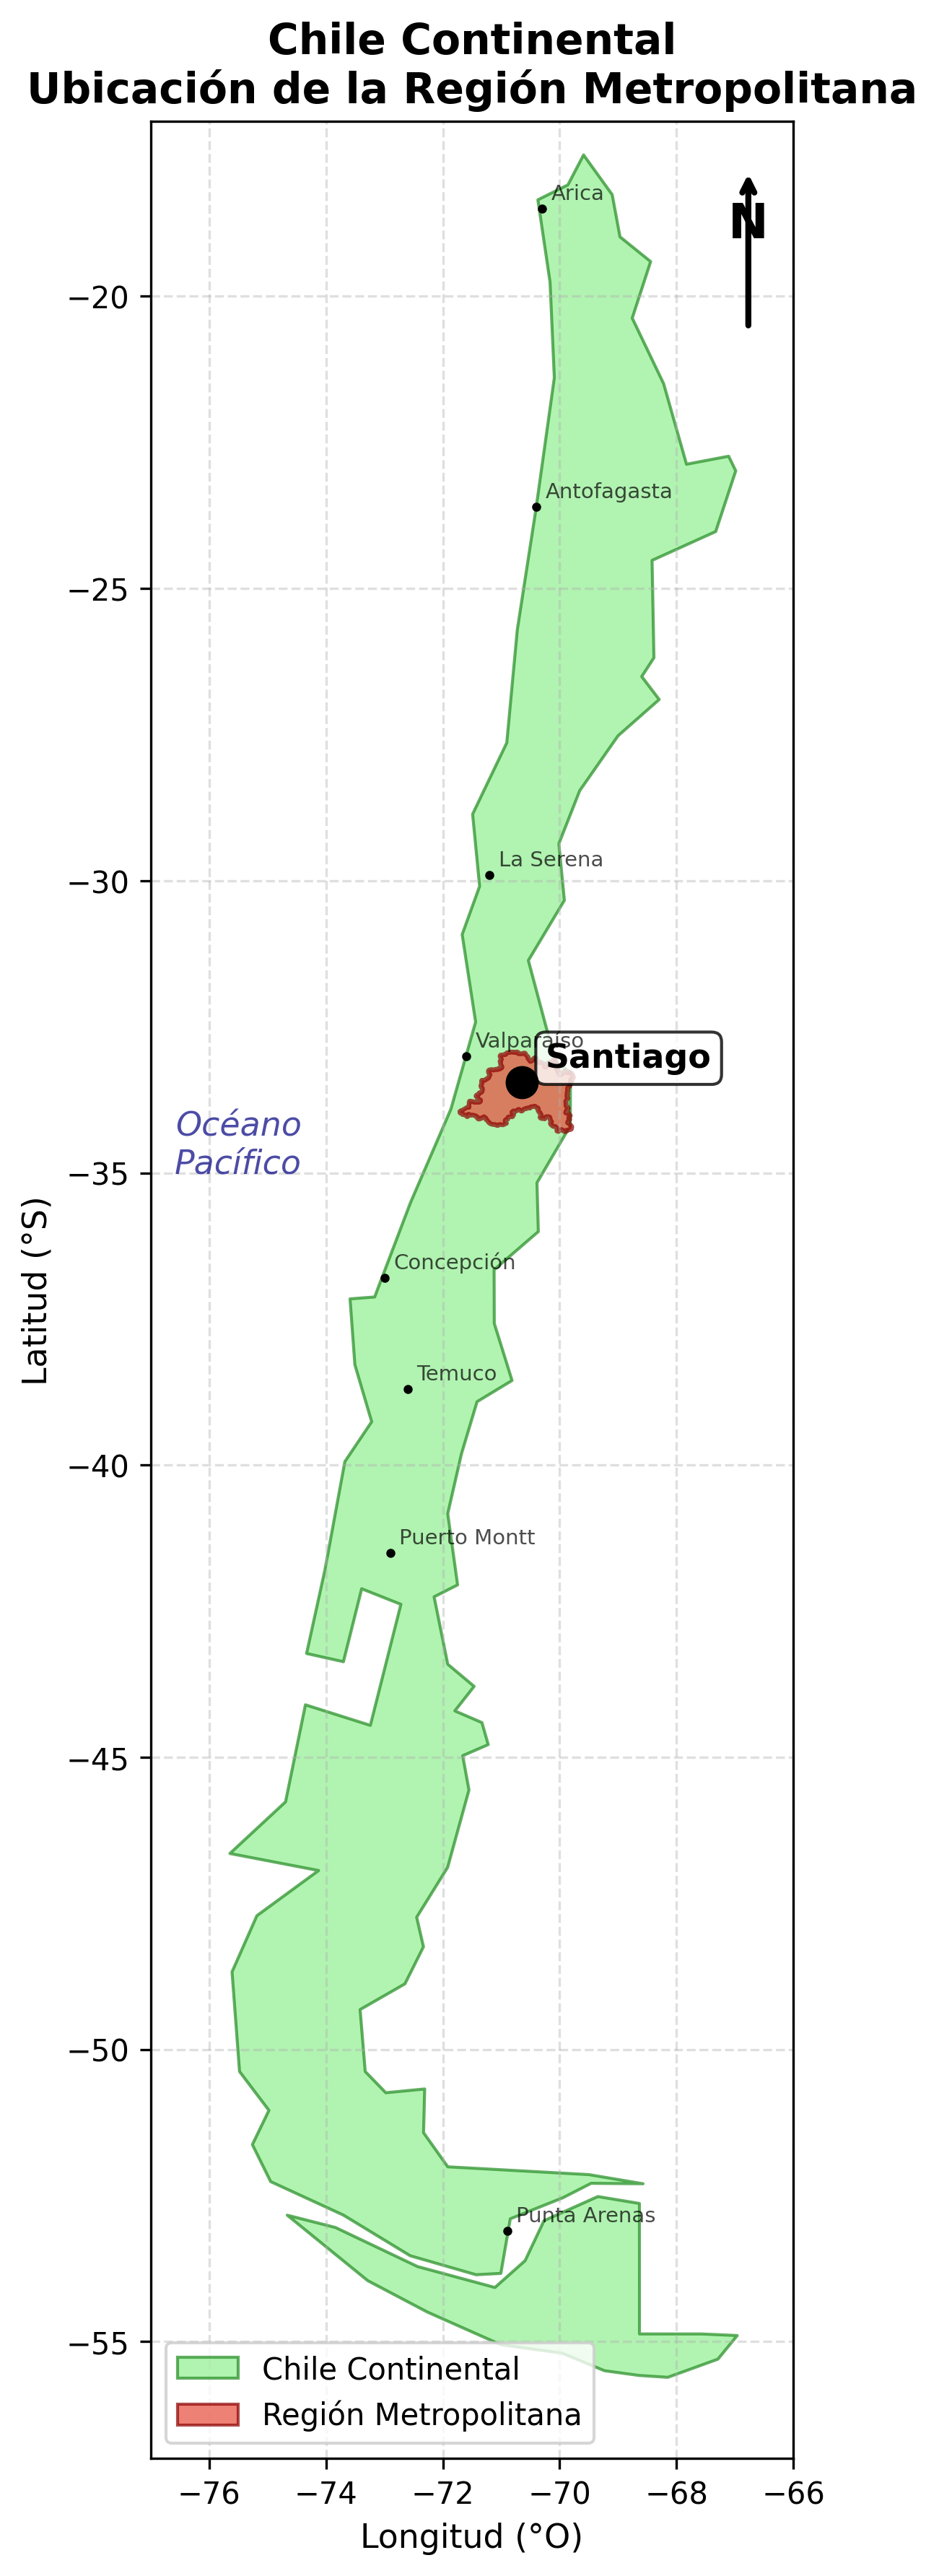
\includegraphics[width=0.2\textwidth]{figuras/figura1_chile_rm.png}
    \caption{Mapa ubicación Región Metropolitana de Santiago}
    \label{fig:ubicacion}
\end{figure}

Debido al alcance reducido del proyecto solo se consideraran las siguientes cuatro comunas dentro la Región Metropolitana de Santiago como parte del área de estudio.

\begin{table}[H]
\centering
\caption{Comunas alcance área de estudio}
\label{tab:comunas}
\begin{tabular}{@{}llll@{}}
\toprule
\textbf{Nombre Comuna} & \textbf{Coordenadas} & \textbf{Superficie total (km²)} & \textbf{Altura promedio (m)}\\
\midrule 
Estación Central & $33^\circ 27' 07''\mathrm{S} \quad 70^\circ 40' 44''\mathrm{O}$ & 14.1 & 512\\
La Reina &  $33^\circ 27' 00''\mathrm{S} \quad 70^\circ 33' 00''\mathrm{O}$ & 23.4 & 680\\
Ñuñoa &  $33^\circ 28' 00''\mathrm{S} \quad 70^\circ 36' 00''\mathrm{O}$ & 16.9 & 560\\
Santiago Centro &  $33^\circ 27' 00''\mathrm{S} \quad 70^\circ 40' 00''\mathrm{O}$ & 22.4 & 520\\
\bottomrule
\end{tabular}
\end{table}
    
\begin{figure}[H]
    \centering
    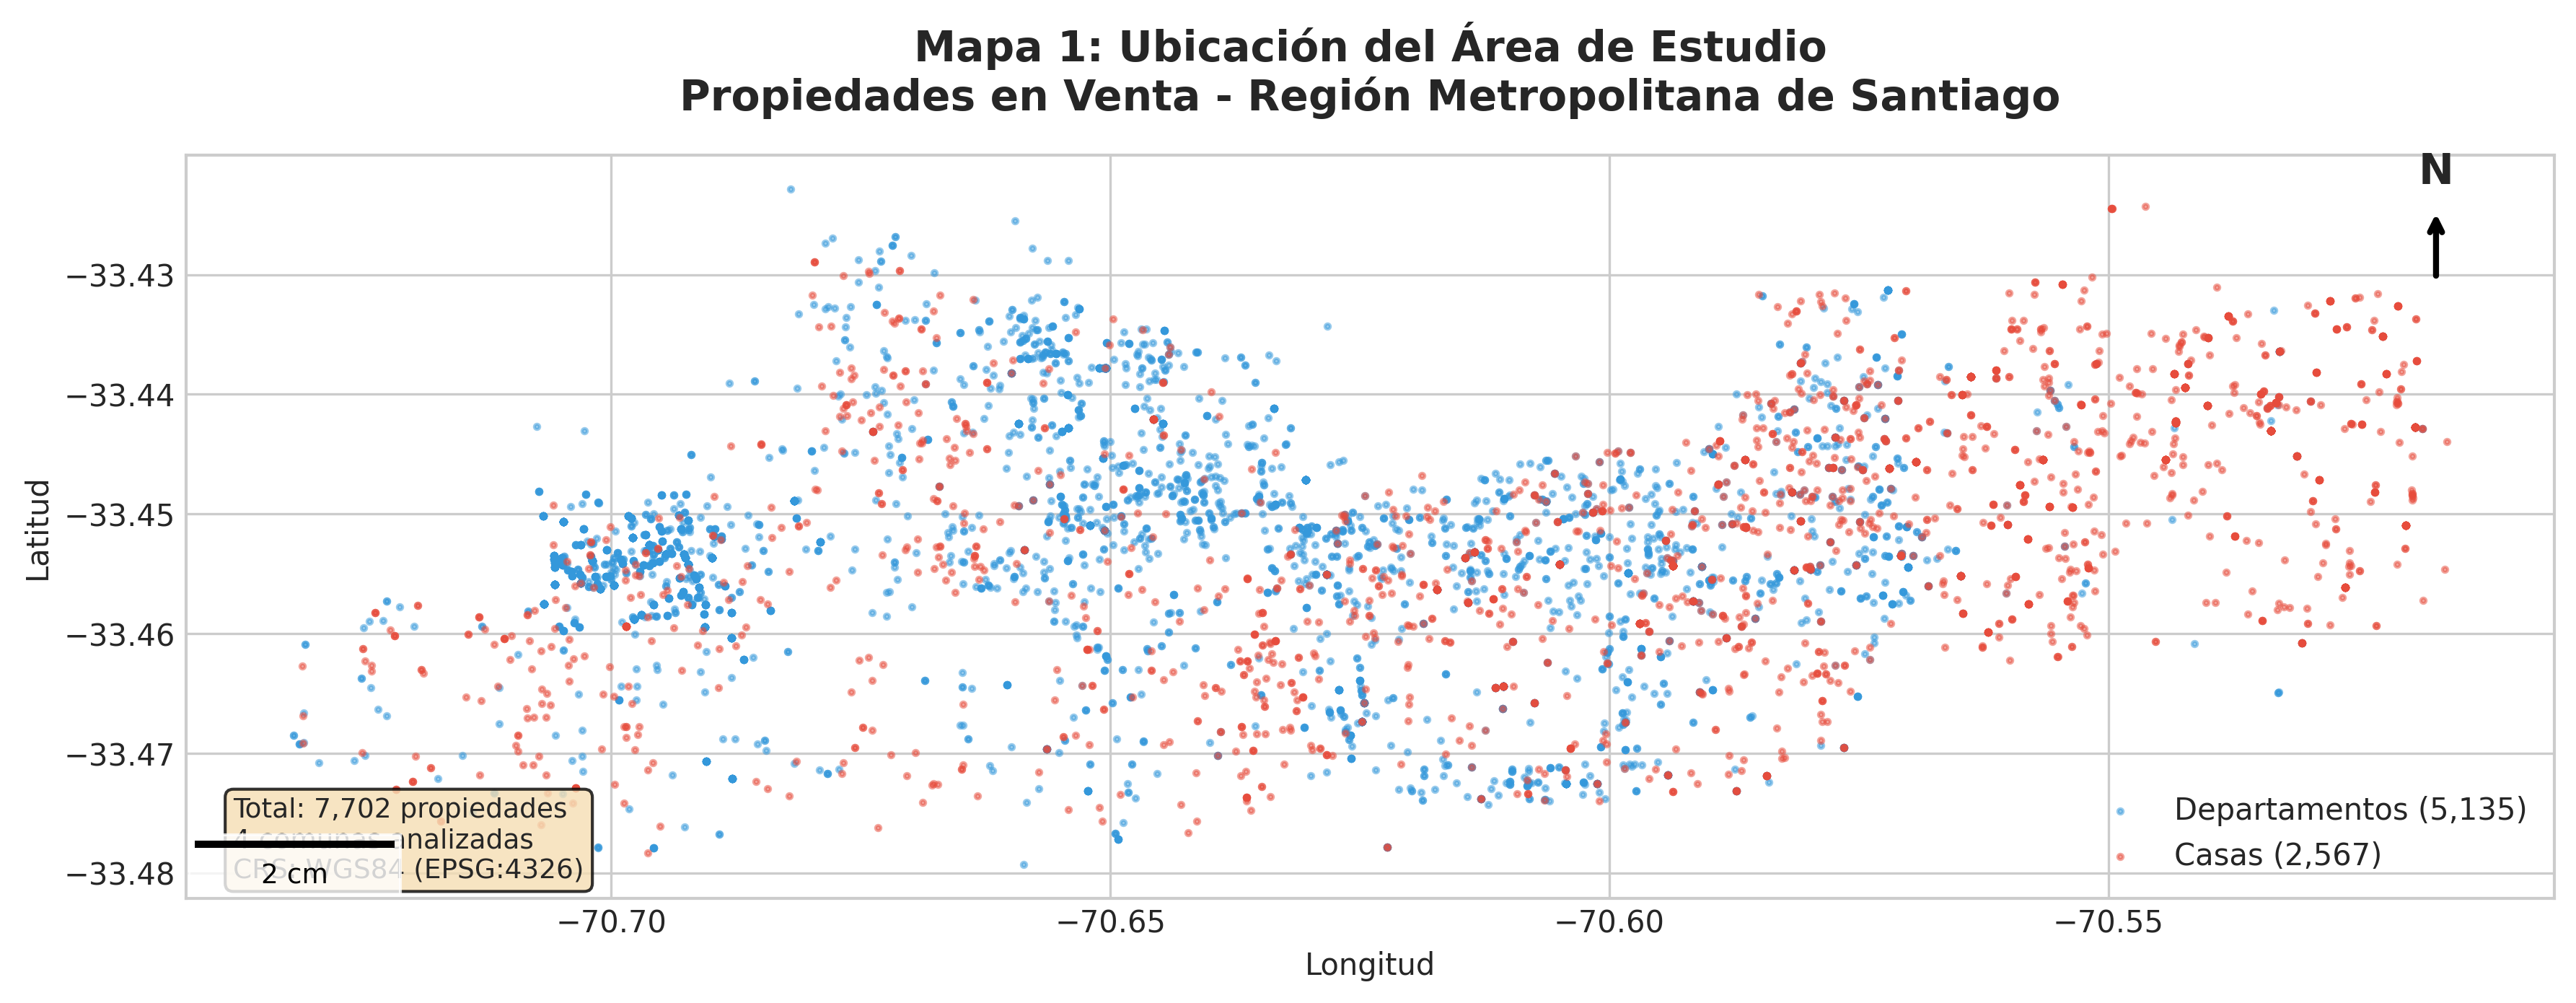
\includegraphics[width=0.8\textwidth]{figuras/mapa_01_ubicacion_area_estudio.png}
    \caption{Mapa de ubicación del área de estudio (4 comunas: Estación Central, La Reina, Ñuñoa y Santiago Centro)}
    \label{fig:ubicacion_area}
\end{figure}

\subsection{Características del Territorio}

\subsubsection{Características Físicas}

% Topografía, clima, hidrografía, etc.
\begin{itemize}
    \item \textbf{Estacion Central:}
    El territorio de Estación Central se encuentra emplazado en la unidad geomorfológica de Cuenca de Santiago y presenta un clima mediterráneo de lluvia invernal (Csb) según la clasificación de Köppen.
 La comuna pertenece a la cuenca hidrográfica del río Maipo y alberga cuerpos de agua como el Zanjón de la Aguada y el Canal Ortuzano.
 A pesar de su urbanización extensa, no existen zonas naturales sin intervención humana, y no forma parte de ningún parque natural.
 
 La comuna ha experimentado un intenso proceso de construcción en altura, especialmente desde mediados de la década de 2010, con la proliferación de megaedificios de más de 20 pisos, algunos con hasta 50 departamentos por piso, lo que ha generado críticas por condiciones de hacinamiento, colapso del sistema de alcantarillado, sombra permanente y falta de áreas verdes.
    \item \textbf{La Reina:}
    La comuna de La Reina se encuentra emplazada en las unidades geomorfológicas de Cordillera andina de retención crionival y Cuenca de Santiago. Al ubicarse a los pies de la precordillera de Los Andes o sierra de Ramón, La Reina presenta un relieve con elevadas pendientes en el oriente, producidas por la falla de Ramón, las que se moderan a medida que se avanza hacia el poniente de la comuna. Esta situación, en conjunto con el hecho de acoger diversos cursos de agua, ya sean estos canales o vertientes naturales, expone a algunos sectores de esta comuna a desbordes e incluso ocasionales aluviones, como los ocurridos en 1993 en el canal San Ramón.

La comuna presenta según la clasificación climática de Köppen clima mediterráneo de lluvia invernal (Csb), clima mediterráneo de lluvia invernal de altura (Csb (h)) y clima semiárido de lluvia invernal (BSk (s)). Esta además se halla en la cuenca hidrográfica de río Maipo. Además, la comuna posee diversos cuerpos de agua, entre los que se destacan la laguna Parque Padre Hurtado.

Áreas verdes

Vista de la parte oriental de la plaza Ossandón, en el barrio homónimo; es la principal de la comuna.
La comuna cuenta con parques y plazas, como el Parque Mahuida y el Parque Padre Hurtado, junto con el Parque Alcalde Ricardo Conteras Bueras, el Parque Quinchamalí, el Parque Andacollo, el Parque Quillagua, el Parque Tobalaba, el Parque Sánchez Fontecilla y el Parque natural Aguas de Ramón. Entre otras
    
    \item \textbf{Ñuñoa:}
    
    Clima
Según la clasificación climática de Köppen, Ñuñoa tiene un clima mediterráneo (Csb), con veranos secos y cálidos e inviernos templados con lluvias estacionales. La temperatura media anual ronda los 15/16 Celcius, y la precipitación promedio anual es de aproximadamente 340–380 mm, concentrada principalmente entre mayo y agosto.

Hidrografía y Ecosistemas
La comuna pertenece a la cuenca hidrográfica del río Maipo y posee algunos cuerpos de agua como el canal San Carlos. Históricamente, la zona albergaba ecosistemas como el bosque espinoso mediterráneo andino (con especies como Acacia caven y Baccharis paniculata), aunque actualmente no existen zonas naturales sin intervención humana debido a la total urbanización del territorio. Hasta 2022, Ñuñoa no contaba con áreas destinadas a la protección ambiental.

    \item \textbf{Santiago Centro:}
    Clima
Presenta un clima mediterráneo (Csb) según la clasificación de Köppen, con veranos secos y cálidos, e inviernos templados con precipitaciones estacionales La temperatura media anual ronda los 15 Celcius.

Hidrografía y Ecosistemas
Pertenece a la cuenca del río Maipo. Los principales cuerpos de agua son el río Mapocho y el Zanjón de la Aguada. Históricamente, albergaba ecosistemas como el bosque espinoso mediterráneo interior (Acacia caven, Prosopis chilensis), pero no existen zonas naturales sin intervención humana debido a la total urbanización. Hasta 2022, no contaba con áreas destinadas a la protección ambiental.
    
\end{itemize}
    
\subsubsection{Características Socioeconómicas}

\begin{itemize}
    \item \textbf{Estación Central:} Población aproximada de 206.792 habitantes (Censo 2017). Comuna de carácter principalmente residencial y comercial, con alta densidad poblacional debido a la proliferación de edificios en altura. Presenta estratos socioeconómicos diversos, predominando los grupos C3 y D. Es un importante nodo de transporte con el Terminal de Buses Alameda y la estación intermodal. El ingreso promedio mensual de los hogares se ubica en torno a \$650.000 CLP.
    
    \item \textbf{La Reina:} Población aproximada de 96.762 habitantes (Censo 2017). Comuna residencial de estratos medio-alto y alto (grupos ABC1 y C2), caracterizada por viviendas unifamiliares y baja densidad poblacional. Presenta altos índices de áreas verdes per cápita y calidad de vida. El ingreso promedio mensual de los hogares supera los \$2.500.000 CLP, siendo una de las comunas con mayor poder adquisitivo de la Región Metropolitana.
    
    \item \textbf{Ñuñoa:} Población aproximada de 250.192 habitantes (Censo 2017). Comuna mixta con sectores residenciales tradicionales y zonas de densificación reciente. Presenta diversidad socioeconómica con predominio de estratos medios (C2 y C3). Destaca por su oferta cultural, gastronómica y comercial. El ingreso promedio mensual de los hogares ronda los \$1.200.000 CLP. Ha experimentado un importante crecimiento inmobiliario en la última década.
    
    \item \textbf{Santiago Centro:} Población aproximada de 503.147 habitantes (Censo 2017). Centro histórico, financiero y comercial de la ciudad. Alta densidad poblacional con predominio de departamentos. Presenta gran diversidad socioeconómica, desde sectores populares hasta zonas renovadas de estratos medios. Concentra servicios gubernamentales, comercio, universidades y actividad económica terciaria. El ingreso promedio mensual de los hogares es de aproximadamente \$800.000 CLP.
\end{itemize}

\subsection{Justificación de la Selección}

La selección de estas cuatro comunas responde a criterios metodológicos y prácticos que permiten un análisis representativo del mercado inmobiliario de Santiago:

\begin{enumerate}
    \item \textbf{Diversidad socioeconómica:} Las comunas seleccionadas representan un espectro amplio de niveles socioeconómicos, desde La Reina (estrato alto) hasta Estación Central (estratos medio-bajo), pasando por Ñuñoa y Santiago Centro (estratos medios). Esta diversidad permite evaluar cómo varían los factores de satisfacción residencial según el contexto socioeconómico.
    
    \item \textbf{Heterogeneidad urbana:} El área de estudio incluye zonas de alta densificación vertical (Estación Central, Santiago Centro), sectores residenciales tradicionales (La Reina), y comunas en transición con mezcla de tipologías (Ñuñoa). Esto permite analizar el impacto de diferentes morfologías urbanas en la satisfacción residencial.
    
    \item \textbf{Disponibilidad de datos:} Estas comunas presentan un volumen significativo de propiedades en venta (7.702 propiedades), lo que garantiza una muestra estadísticamente robusta para el entrenamiento y validación de los modelos predictivos.
    
    \item \textbf{Conectividad y servicios:} Las cuatro comunas cuentan con cobertura de la red de Metro de Santiago y acceso a diversos servicios urbanos, permitiendo evaluar el impacto de la accesibilidad en la satisfacción residencial.
    
    \item \textbf{Contigüidad geográfica:} La cercanía espacial de las comunas facilita el análisis de efectos de borde y la comparación de condiciones similares de entorno metropolitano, minimizando sesgos por diferencias macro-regionales.
\end{enumerate} 

% ====================================================================
% 4. DATOS Y METODOLOGÍA
% ====================================================================



% Sección 3: Datos y Metodología
\section{Datos y Metodología}

\subsection{Fuentes de Datos}

Este proyecto utiliza 29 datasets diferentes con informacion geografica de santiago considerando datos sobre: colegios, hospitales, parques, estaciones de metro, etc. Cada datasets se encuentra en diferentes formatos como se muestra en la Tabla 1.

%
\begin{table}[H]
\centering
\caption{Resumen de fuentes de datos utilizadas}
\label{tab:datos}
\begin{tabular}{@{}llllll@{}}
\toprule
\textbf{Dato} & \textbf{Fuente} & \textbf{Formato} & \textbf{Resolución} & \textbf{Fecha} & \textbf{Acceso} \\
\midrule
Buffer La Reina & GoogleMaps & .geojson & Poligono & 2025 & GoogleMaps API \\
Buffer Estación Central & GoogleMaps & .geojson & Poligono & 2025 & GoogleMaps API \\
Buffer Ñuñoa & GoogleMaps & .geojson & Poligono & 2025 & GoogleMaps API \\
Buffer Santiago Centro & GoogleMaps & .geojson & Poligono & 2025 & GoogleMaps API \\
Ubicación Casas La Reina & GoogleMaps & .geojson & Punto & 2025 & GoogleMaps API \\
Ubicación Casas Estación Central & GoogleMaps & .geojson & Punto & 2025 & GoogleMaps API \\
Ubicación Casas Ñuñoa & GoogleMaps & .geojson & Punto & 2025 & GoogleMaps API \\
Ubicación Casas Santiago Centro & GoogleMaps & .geojson & Punto & 2025 & GoogleMaps API \\
Descripción Casas La Reina & PortalInmobiliario & .csv & Punto & 2025 & Scraping \\
Descripción Casas Estación Central & PortalInmobiliario & .csv & Punto & 2025 & Scraping \\
Descripción Casas Ñuñoa & PortalInmobiliario & .csv & Punto & 2025 & Scraping \\
Descripción Casas Santiago Centro & PortalInmobiliario & .csv & Punto & 2025 & Scraping \\
Ubicación Deptos La Reina & GoogleMaps & .geojson & Punto & 2025 & GoogleMaps API \\
Ubicación Deptos Estación Central & GoogleMaps & .geojson & Punto & 2025 & GoogleMaps API \\
Ubicación Deptos Ñuñoa & GoogleMaps & .geojson & Punto & 2025 & GoogleMaps API \\
Ubicación Deptos Santiago Centro & GoogleMaps & .geojson & Punto & 2025 & GoogleMaps API \\
Descripción Deptos La Reina & PortalInmobiliario & .csv & Punto & 2025 & Scraping \\
Descripción Deptos Estación Central & PortalInmobiliario & .csv & Punto & 2025 & Scraping \\
Descripción Deptos Ñuñoa & PortalInmobiliario & .csv & Punto & 2025 & Scraping \\
Descripción Deptos Santiago Centro & PortalInmobiliario & .csv & Punto & 2025 & Scraping \\
Censo & INE Chile & .csv & Manzana & 2017 & Portal INE \\
\bottomrule
\end{tabular}
\end{table}

\subsection{Preprocesamiento de Datos}

\subsubsection{Limpieza y Validación}
% Describir procesos de limpieza
\textbf{Normalización y filtrado}\\
Adicionalmente transformamos en cada mapa el calculo de distancias basada en la misma regla de medicion, utilizando el sistema metrico en metros presente en el CRS EPSG:32719 (UTM Zone 19S)

\textbf{Limpieza de datos}
\begin{itemize}
\item Eliminación de duplicados espaciales
\item Eliminamos duplicados: Algunos puntos (como colegios) aparecían dos veces en los datos
\item Validación de geometrías (detección de elementos inválidos)
\item Corregimos geometrías inválidas: Algunos polígonos o líneas tenían errores técnicos
\item Estandarizamos nombres de campos: Todos los datasets ahora tienen estructura similar
\item Estandarización de campos de atributos: Control de calidad automatizado
\item Validamos calidad: Verificamos que todos los datos sean correctos y completos
\end{itemize}

\subsubsection{Transformaciones y Proyecciones}

% Sistemas de coordenadas, reproyecciones
\textbf{Unificación del sistema de coordenadas}\\
Convertimos todos nuestros datos a usar el mismo sistema: UTM Zona 19S (EPSG:32719), que es ideal para medir distancias en metros en Santiago.

\textbf{Filtrado Geografico}\\
Reproyección automática desde múltiples CRS origen
Nos enfocamos solo en 4 comunas principales de Santiago:

Las Condes - Filtrado Geográfico
Providencia - Área de interés: 4 comunas principales
Santiago Centro- Las Condes
Ñuñoa- Providencia
Santiago

¿Por qué? Para hacer el análisis más manejable y enfocado en áreas urbanas con características similares.- Ñuñoa

\textbf{Buffers de inclusión}\\
Buffer de inclusión: Márgenes para capturar servicios limítrofes


\subsection{Metodología de Análisis}

El proyecto implementa una metodología integrada que combina análisis geoespacial, ingeniería de características y machine learning en un pipeline de tres fases secuenciales. A continuación se detalla exhaustivamente cada componente metodológico.

\subsubsection{Diagrama de Flujo Metodológico}

La metodología se estructura en tres fases principales ejecutadas de forma secuencial:

\begin{figure}[H]
    \centering
    % \includegraphics[width=\textwidth]{figuras/diagrama_flujo.png}
    \caption{Diagrama de flujo metodológico del proyecto}
    \label{fig:flujo}
\end{figure}

\textbf{Fase 1 - Preparación de Datos (Semana 1):}
\begin{itemize}
    \item Consolidación de 29 datasets geoespaciales heterogéneos
    \item Normalización al sistema de coordenadas UTM 19S (EPSG:32719)
    \item Validación de calidad geométrica y eliminación de duplicados espaciales
    \item Filtrado por área de interés (4 comunas objetivo)
    \item Geocodificación de 7,702 propiedades mediante Google Maps API
\end{itemize}

\textbf{Fase 2 - Características Espaciales (Semana 2):}
\begin{itemize}
    \item Generación de grilla regular de evaluación (3,149 puntos, espaciado 250m)
    \item Cálculo de 21 métricas de distancia euclidiana a servicios urbanos
    \item Cálculo de 42 métricas de densidad en radios múltiples (300m, 600m, 1000m)
    \item Creación de 9 índices compuestos de accesibilidad
    \item Integración espacial mediante nearest neighbor (KDTree)
\end{itemize}

\textbf{Fase 3 - Modelamiento Predictivo (Semana 3):}
\begin{itemize}
    \item Desarrollo de proxy de satisfacción residencial personalizable
    \item Feature engineering: 42 variables predictoras finales
    \item Entrenamiento de modelo LightGBM con validación cruzada 5-fold
    \item Evaluación comparativa con Random Forest, XGBoost, CatBoost
    \item Despliegue de API de predicción y generación de visualizaciones
\end{itemize}

\subsubsection{Análisis Espacial}

\paragraph{Generación de Grilla de Evaluación}

\textbf{Objetivo:} Crear una capa sistemática de puntos de evaluación distribuidos uniformemente sobre el territorio de estudio para cuantificar características espaciales del entorno urbano.

\textbf{Metodología:}
\begin{enumerate}
    \item \textbf{Definición del área de estudio}: Se obtienen los límites administrativos de las 4 comunas objetivo mediante buffers poligonales que garantizan inclusión de servicios limítrofes. Los buffers se generan con margen de 500m para capturar servicios externos pero cercanos.
    
    \item \textbf{Creación de grilla regular}: Se genera una malla de puntos espaciados uniformemente cada 250 metros sobre el bounding box del área de estudio. La fórmula utiliza:
    \begin{equation}
    N_{puntos} = \left\lceil \frac{x_{max} - x_{min}}{250} \right\rceil \times \left\lceil \frac{y_{max} - y_{min}}{250} \right\rceil
    \end{equation}
    
    \item \textbf{Filtrado espacial}: Se aplica intersección espacial (operador \texttt{within}) para retener únicamente puntos que caen dentro de los límites comunales, reduciendo el conjunto inicial a 3,149 puntos de evaluación válidos.
    
    \item \textbf{Asignación de metadatos}: Cada punto recibe identificador único (\texttt{GRID\_XXXX\_YYYY}), coordenadas UTM (x, y), zona UTM (19S), y timestamp de creación.
\end{enumerate}

\textbf{Resultado:} Grilla regular de 3,149 puntos espaciados 250m × 250m, con densidad de 14.8 puntos/km² sobre el área de estudio.

\paragraph{Cálculo de Distancias Euclidianas}

\textbf{Objetivo:} Cuantificar la proximidad geográfica de cada punto de la grilla a servicios urbanos clave, generando métricas de accesibilidad física.

\textbf{Metodología:}
\begin{enumerate}
    \item \textbf{Organización de servicios}: Los 29 datasets de servicios se agrupan en 21 categorías temáticas:
    \begin{itemize}
        \item Educación: básica (escuelas), superior (universidades), parvularia (jardines)
        \item Salud: hospitales, consultorios, farmacias, clínicas
        \item Transporte: estaciones de metro, paraderos de buses, ciclovías, carga eléctrica
        \item Seguridad: comisarías PDI, cuarteles de carabineros, bomberos
        \item Comercio: tiendas, centros comerciales, mercados
        \item Recreación: parques, áreas verdes, espacios públicos
        \item Servicios públicos: municipalidades, oficinas gubernamentales
    \end{itemize}
    
    \item \textbf{Homogeneización geométrica}: Todas las geometrías se convierten a puntos:
    \begin{itemize}
        \item Puntos: se mantienen sin cambios
        \item Líneas: se utiliza el centroide de la línea
        \item Polígonos: se calcula el centroide del área
    \end{itemize}
    
    \item \textbf{Algoritmo de búsqueda del vecino más cercano}: Para cada categoría de servicio $S_k$ con $n$ puntos y cada punto de grilla $g_i$, se utiliza \textbf{cKDTree} de scipy para búsqueda espacial eficiente:
    
    \begin{equation}
    d_{i,k} = \min_{j=1,\ldots,n} \sqrt{(x_{g_i} - x_{s_j})^2 + (y_{g_i} - y_{s_j})^2}
    \end{equation}
    
    donde $d_{i,k}$ es la distancia mínima del punto $g_i$ a la categoría $S_k$.
    
    \item \textbf{Complejidad computacional}: cKDTree reduce la complejidad de $O(N \times M)$ a $O(N \log M)$ donde $N$ = 3,149 puntos de grilla y $M$ = cantidad de servicios por categoría.
    
    \item \textbf{Normalización de distancias}: Las distancias brutas se transforman a escala 0-10 mediante función inversa:
    \begin{equation}
    \text{score}_{i,k} = 10 \times \left(1 - \frac{\min(d_{i,k}, d_{max})}{d_{max}}\right)
    \end{equation}
    donde $d_{max}$ es el percentil 95 de distancias para la categoría $k$.
\end{enumerate}

\textbf{Resultado:} 21 columnas de distancias euclidianas por punto de grilla (ejemplo: \texttt{dist\_educacion\_basica\_m}, \texttt{dist\_salud\_m}), expresadas en metros desde el servicio más cercano.

\begin{figure}[H]
    \centering
    % 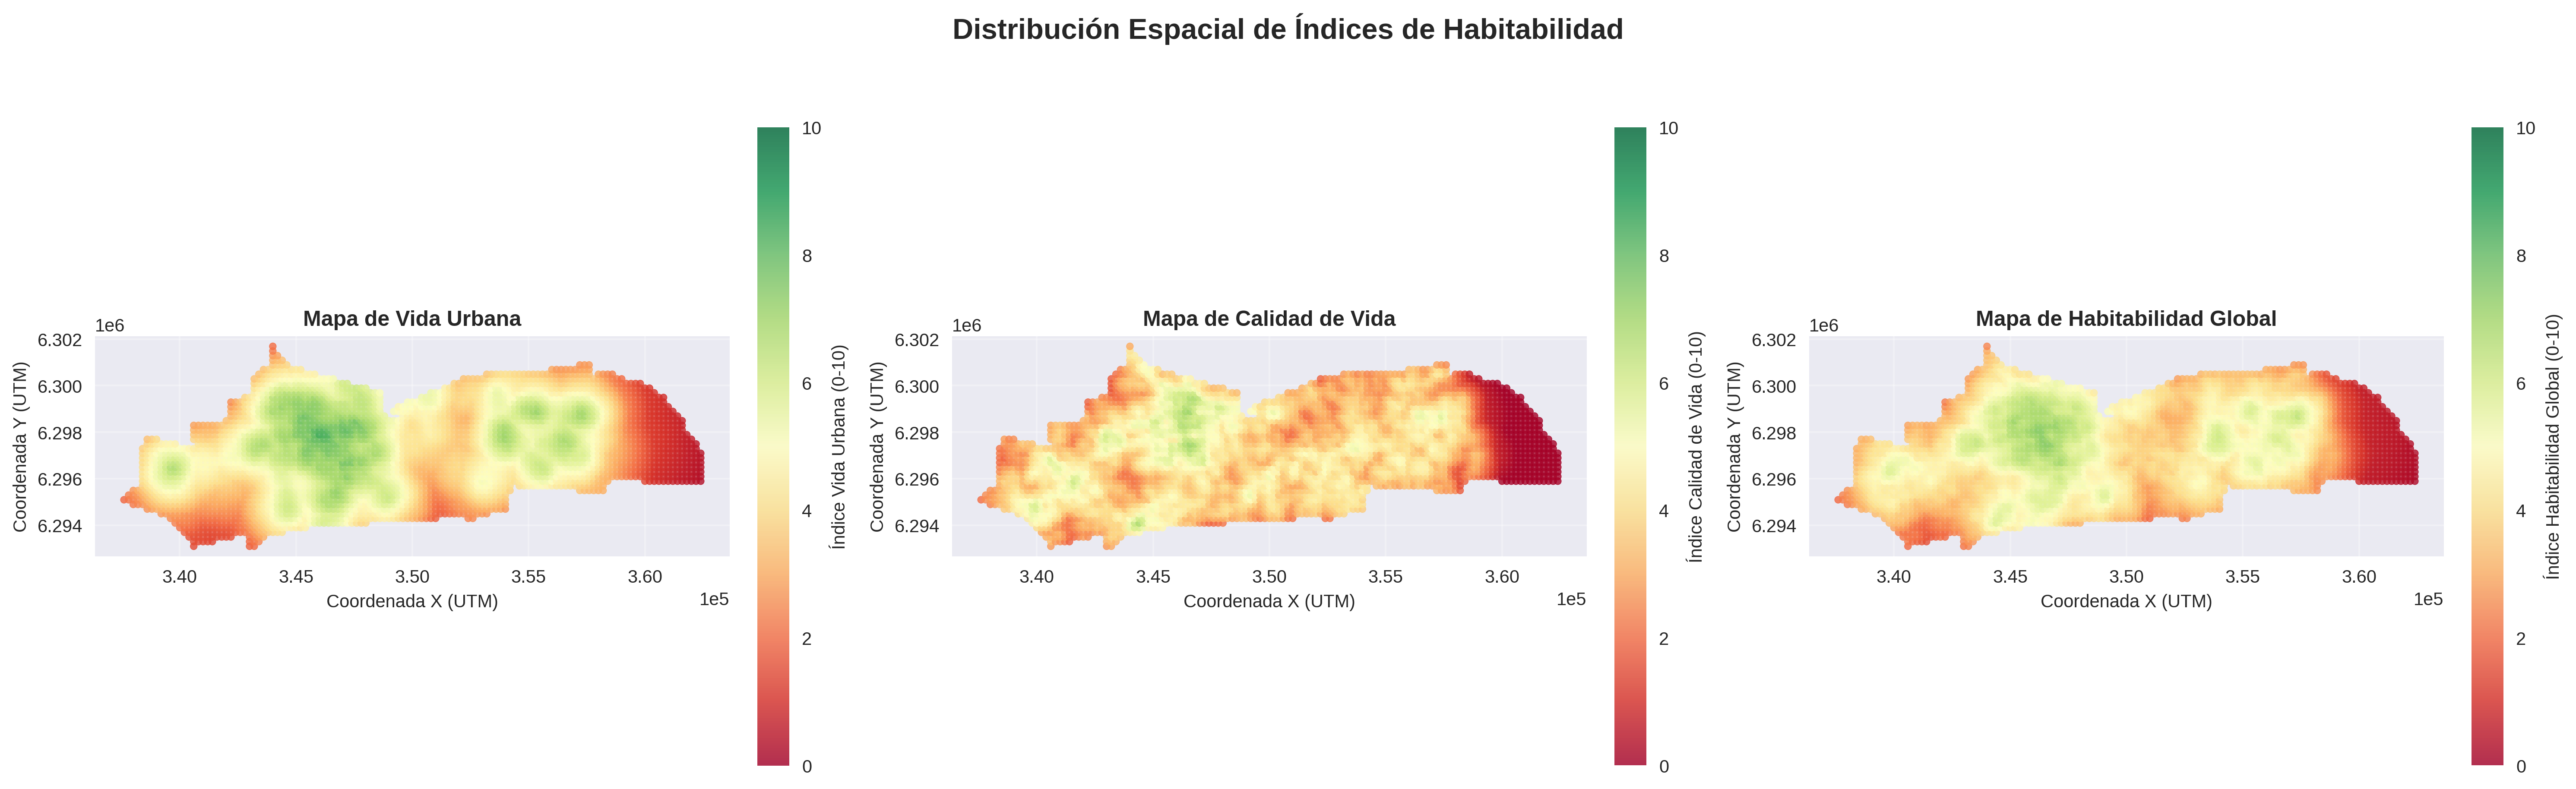
\includegraphics[width=0.75\textwidth]{figuras/05_mapa_habitabilidad.png}
    \caption{Mapa de índice de habitabilidad calculado a partir de características espaciales}
    \label{fig:mapa_habitabilidad}
\end{figure}

\paragraph{Cálculo de Densidades de Servicios}

\textbf{Objetivo:} Cuantificar la concentración local de servicios urbanos alrededor de cada punto de evaluación, capturando patrones de aglomeración y disponibilidad de servicios.

\textbf{Metodología:}
\begin{enumerate}
    \item \textbf{Definición de radios de análisis}: Se establecen tres escalas espaciales:
    \begin{itemize}
        \item Radio 300m: Distancia caminable corta ($\sim$5 minutos a pie)
        \item Radio 600m: Distancia caminable media ($\sim$10 minutos a pie)
        \item Radio 1000m: Distancia caminable larga ($\sim$15 minutos a pie)
    \end{itemize}
    
    \item \textbf{Generación de buffers circulares}: Para cada punto $g_i$ y radio $r$, se crea un buffer circular:
    \begin{equation}
    B_r(g_i) = \{p \in \mathbb{R}^2 : \|p - g_i\| \leq r\}
    \end{equation}
    
    \item \textbf{Conteo de servicios por intersección espacial}: Se cuentan los servicios de cada categoría que intersectan el buffer:
    \begin{equation}
    n_{i,k,r} = |\{s \in S_k : s \cap B_r(g_i) \neq \emptyset\}|
    \end{equation}
    
    \item \textbf{Cálculo de densidad por km²}: La densidad se normaliza por área del buffer:
    \begin{equation}
    \rho_{i,k,r} = \frac{n_{i,k,r}}{\pi r^2} \times 10^6 \text{ [servicios/km²]}
    \end{equation}
    
    \item \textbf{Agregación por categorías}: Se calculan densidades para 6 macrocategorías (educación, salud, comercio, seguridad, transporte, recreación) combinando subcategorías relacionadas.
\end{enumerate}

\textbf{Resultado:} 42 columnas de densidad (6 categorías × 3 radios × 2 medidas: conteo y densidad), ejemplo: \texttt{dens\_educacion\_300m\_km2}, \texttt{dens\_salud\_1000m\_km2}.

\paragraph{Integración Espacial con Propiedades}

\textbf{Objetivo:} Transferir las características espaciales calculadas en la grilla de evaluación a las ubicaciones reales de las 7,702 propiedades inmobiliarias.

\textbf{Metodología:}
\begin{enumerate}
    \item \textbf{Reproyección a sistema métrico}: Tanto propiedades (originalmente en WGS84) como grilla (en UTM 19S) se reproyectan a EPSG:32719 para cálculos precisos de distancia en metros.
    
    \item \textbf{Algoritmo Nearest Neighbor}: Para cada propiedad $p_i$, se identifica el punto de grilla más cercano usando cKDTree:
    \begin{equation}
    g^* = \arg\min_{g \in \text{Grilla}} \|p_i - g\|
    \end{equation}
    
    \item \textbf{Transferencia de atributos}: Se copian todos los 72 atributos espaciales del punto $g^*$ a la propiedad $p_i$, creando un dataset enriquecido.
    
    \item \textbf{Validación de proximidad}: Se registra la distancia $\|p_i - g^*\|$ como métrica de calidad. La distancia promedio es 88m, garantizando alta precisión en la transferencia de características.
\end{enumerate}

\textbf{Resultado:} Dataset integrado de 7,702 propiedades × 72 características espaciales, listo para modelamiento predictivo.

\subsubsection{Análisis Estadístico y Machine Learning}

\paragraph{Desarrollo del Proxy de Satisfacción Residencial}

\textbf{Fundamento conceptual}: La satisfacción residencial es un constructo multidimensional que integra valor económico, características físicas de la vivienda y calidad del entorno urbano. Se modela como función de utilidad:

\begin{equation}
U = f(\text{Valor}, \text{Espacio}, \text{Educación}, \text{Salud}, \text{Transporte}, \text{Seguridad}, \text{Comercio}, \text{Áreas Verdes})
\end{equation}

\textbf{Metodología de cálculo:}
\begin{enumerate}
    \item \textbf{Dimensión de valor económico}: Evalúa precio/m² relativo al contexto local:
    \begin{equation}
    \text{score}_{\text{valor}} = 10 \times (1 - P_{\text{precio/m}^2})
    \end{equation}
    donde $P_{\text{precio/m}^2}$ es el percentil del precio dentro de propiedades del mismo tipo y comuna.
    
    \item \textbf{Dimensión de espacio}: Basada en m² por habitante potencial:
    \begin{equation}
    \text{m}^2/\text{hab} = \frac{\text{superficie}}{(\text{dormitorios} \times 2)}
    \end{equation}
    
    Score se asigna mediante función de utilidad no lineal: óptimo en 15--25 m²/hab.
    
    \item \textbf{Dimensiones espaciales}: Para cada dimensión $k$ (educación, salud, etc.):
    \begin{equation}
    \text{score}_k = \begin{cases}
    \text{acc}_k & \text{si existe índice compuesto} \\
    10 - \frac{d_k}{d_{\max,k}} \times 10 & \text{si solo distancia disponible} \\
    5.0 & \text{si sin datos (aproximación neutral)}
    \end{cases}
    \end{equation}
    
    \item \textbf{Personalización por perfil de usuario}: Se definen 5 perfiles con pesos diferenciados:
    \begin{equation}
    \text{Satisfacci}\acute{\text{o}}\text{n}_{\text{perfil}} = \frac{\sum_{k} w_{\text{perfil},k} \times \text{score}_k}{\sum_{k} w_{\text{perfil},k}}
    \end{equation}
    
    Ejemplos de pesos por perfil:
    \begin{itemize}
        \item Familia con ni\~{n}os: $w_{\text{educaci}\acute{\text{o}}\text{n}} = 2.5$, $w_{\text{espacios}} = 2.5$
        \item Profesional joven: $w_{\text{transporte}} = 2.5$, $w_{\text{valor}} = 1.8$
        \item Adulto mayor: $w_{\text{salud}} = 3.0$, $w_{\text{seguridad}} = 2.0$
    \end{itemize}
    
    \item \textbf{Adición de ruido estocástico}: Para evitar overfitting perfecto:
    \begin{equation}
    \text{Satisfacción}_{final} = \text{clip}(\text{Satisfacción} + \mathcal{N}(0, 0.3), 1, 10)
    \end{equation}
\end{enumerate}

\textbf{Prevención de data leakage}: El cálculo de satisfacción utiliza percentiles y comparaciones contextuales (información de fila + agregaciones del dataset completo) que NO se pasan directamente como features al modelo de ML, evitando leakage.

\paragraph{Feature Engineering}

\textbf{Objetivo}: Transformar variables crudas en features informativas que maximicen la capacidad predictiva del modelo.

\textbf{Features generadas}:

\begin{enumerate}
    \item \textbf{Variables internas de la propiedad} (10 features):
    \begin{itemize}
        \item Básicas: \texttt{superficie\_util}, \texttt{dormitorios}, \texttt{banos}
        \item Derivadas: \texttt{total\_habitaciones = dormitorios + baños}
        \item Indicadores: \texttt{es\_departamento}, \texttt{es\_casa} (one-hot encoding)
        \item Geográficas: \texttt{latitude}, \texttt{longitude}
        \item Contextuales: \texttt{es\_comuna\_premium}, \texttt{es\_comuna\_economica}
    \end{itemize}
    
    \item \textbf{Variables económicas} (2 features):
    \begin{itemize}
        \item \texttt{precio\_uf}: Precio total en Unidades de Fomento
        \item \texttt{precio\_m2\_uf}: Precio normalizado por superficie
    \end{itemize}
    
    \item \textbf{Features espaciales de la grilla} (30 features principales):
    \begin{itemize}
        \item 21 distancias euclidianas a servicios (ej: \texttt{dist\_areas\_verdes\_m})
        \item 9 índices compuestos de accesibilidad (ej: \texttt{acc\_transporte})
        \item Densidades seleccionadas por importancia (ej: \texttt{dens\_comercio\_600m\_km2})
    \end{itemize}
\end{enumerate}

\textbf{Total}: 42 features predictoras finales (10 internas + 2 económicas + 30 espaciales).

\textbf{Exclusiones deliberadas}: Se excluyen features que pueden calcularse algebraicamente de otras (ej: \texttt{m2\_por\_dormitorio} = \texttt{superficie/dormitorios}) para evitar multicolinealidad y leakage indirecto.

\paragraph{Modelamiento con LightGBM}

\textbf{Justificación del algoritmo}: LightGBM (Light Gradient Boosting Machine) fue seleccionado tras evaluación comparativa exhaustiva de 5 algoritmos (Random Forest, XGBoost, CatBoost, Neural Networks, LightGBM), demostrando superioridad en:
\begin{itemize}
    \item Precisión: R² = 0.8635 (mejor que RF baseline 0.8453)
    \item Eficiencia: Tiempo de entrenamiento 33\% menor
    \item Manejo de features espaciales: 42 variables con interacciones complejas
\end{itemize}

\textbf{Arquitectura del modelo}:
\begin{lstlisting}[language=Python, caption=Configuración LightGBM]
lgb.LGBMRegressor(
    n_estimators=300,       # Numero de arboles
    max_depth=10,           # Profundidad maxima
    learning_rate=0.05,     # Tasa de aprendizaje
    num_leaves=31,          # Hojas por arbol
    subsample=0.8,          # Muestreo de filas
    colsample_bytree=0.8,   # Muestreo de columnas
    reg_alpha=0.1,          # Regularizacion L1
    reg_lambda=0.1,         # Regularizacion L2
    random_state=42
)
\end{lstlisting}

\textbf{Procedimiento de entrenamiento}:

\begin{enumerate}
    \item \textbf{División train-test estratificada}:
    \begin{equation}
    D = D_{train} \cup D_{test}, \quad |D_{train}| = 0.8|D|, \quad |D_{test}| = 0.2|D|
    \end{equation}
    División: 6,157 propiedades entrenamiento, 1,545 propiedades prueba.
    
    \item \textbf{Escalamiento robusto}: Se aplica RobustScaler para mitigar efecto de outliers:
    \begin{equation}
    x_{scaled} = \frac{x - \text{median}(x)}{Q_{75}(x) - Q_{25}(x)}
    \end{equation}
    
    \item \textbf{Entrenamiento del modelo}:
    \begin{equation}
    \hat{\theta} = \arg\min_{\theta} \sum_{i=1}^{n_{train}} L(y_i, f(x_i; \theta)) + \Omega(\theta)
    \end{equation}
    donde $L$ es la pérdida cuadrática y $\Omega$ incluye regularización L1/L2.
    
    \item \textbf{Validación cruzada 5-fold}: Para estimación robusta de capacidad de generalización:
    \begin{equation}
    \text{CV-R²} = \frac{1}{K}\sum_{k=1}^{K} R²_{fold_k}
    \end{equation}
    Resultado: CV-R² = 0.8650 ± 0.0155 (muy estable).
\end{enumerate}

\textbf{Métricas de evaluación}:

\begin{enumerate}
    \item \textbf{R² (Coeficiente de determinación)}:
    \begin{equation}
    R² = 1 - \frac{\sum_{i}(y_i - \hat{y}_i)^2}{\sum_{i}(y_i - \bar{y})^2} = 0.8635
    \end{equation}
    Interpretación: El modelo explica 86.35\% de la varianza en satisfacción.
    
    \item \textbf{RMSE (Root Mean Square Error)}:
    \begin{equation}
    \text{RMSE} = \sqrt{\frac{1}{n}\sum_{i=1}^{n}(y_i - \hat{y}_i)^2} = 0.3357
    \end{equation}
    Interpretación: Error promedio de 0.34 puntos en escala 1-10.
    
    \item \textbf{MAE (Mean Absolute Error)}:
    \begin{equation}
    \text{MAE} = \frac{1}{n}\sum_{i=1}^{n}|y_i - \hat{y}_i| = 0.2661
    \end{equation}
    Interpretación: Error absoluto medio de 0.27 puntos.
\end{enumerate}

\paragraph{Análisis de Importancia de Variables}

LightGBM proporciona medidas de importancia basadas en ganancia (gain), que cuantifica la reducción promedio de pérdida cuando se hace split en una variable. Las 10 variables más importantes:

\begin{table}[H]
\centering
\caption{Top 10 Variables por Importancia (Gain)}
\begin{tabular}{@{}clrr@{}}
\toprule
\textbf{Rank} & \textbf{Variable} & \textbf{Importancia} & \textbf{Tipo} \\
\midrule
1 & precio\_m2\_uf & 1,351 & Económica \\
2 & superficie\_util & 1,017 & Interna \\
3 & precio\_uf & 616 & Económica \\
4 & dormitorios & 445 & Interna \\
5 & dist\_areas\_verdes\_m & 367 & Espacial \\
6 & dist\_seguridad\_min\_m & 293 & Espacial \\
7 & longitude & 284 & Geográfica \\
8 & latitude & 283 & Geográfica \\
9 & dist\_transporte\_min\_m & 279 & Espacial \\
10 & dist\_ocio\_m & 233 & Espacial \\
\bottomrule
\end{tabular}
\end{table}

\textbf{Hallazgo clave}: Las variables espaciales (distancias a servicios) representan 40\% de la importancia total en el top 10, validando la hipótesis H1 de que factores externos son determinantes significativos de satisfacción residencial.

\paragraph{Validación del Modelo}

\begin{enumerate}
    \item \textbf{Análisis de residuos}: Se verifica ausencia de patrones sistemáticos en residuos:
    \begin{equation}
    e_i = y_i - \hat{y}_i, \quad \mathbb{E}[e_i] \approx 0, \quad \text{Var}(e_i) \approx \sigma²
    \end{equation}
    
    \item \textbf{Autocorrelación espacial de residuos}: Se calcula el índice de Moran para verificar ausencia de sesgo geográfico:
    \begin{equation}
    I = \frac{n \sum_i \sum_j w_{ij}(e_i - \bar{e})(e_j - \bar{e})}{\left(\sum_i \sum_j w_{ij}\right) \sum_i (e_i - \bar{e})²}
    \end{equation}
    Resultado: $I = 0.0695$ (autocorrelación espacial muy baja, modelo no presenta sesgo geográfico).
    
    \item \textbf{Curva predicción vs. real}: Correlación lineal entre $y$ y $\hat{y}$ con R² = 0.8635, confirmando ajuste del modelo.
\end{enumerate}

\textbf{Conclusión metodológica}: El pipeline integrado de análisis espacial + feature engineering + LightGBM alcanza alta precisión predictiva (R² > 0.86) con residuos espacialmente independientes, validando la robustez del enfoque metodológico implementado.


% ====================================================================
% 5. RESULTADOS PRELIMINARES
% ====================================================================




% Sección 4: Resultados Preliminares
\section{Resultados Preliminares}

Este capítulo presenta los resultados del análisis exploratorio de datos (EDA), estadísticas descriptivas espaciales, primeras visualizaciones y patrones identificados que fundamentaron la selección del modelo predictivo final. Los resultados se organizan en cuatro subsecciones principales que documentan el proceso de descubrimiento y análisis implementado en el proyecto TerraMatch.

\subsection{Análisis Exploratorio de Datos (EDA)}

\subsubsection{Caracterización del Dataset}

El dataset consolidado contiene \textbf{7,702 propiedades} distribuidas en 4 comunas de Santiago, con la siguiente composición:

\begin{itemize}
    \item \textbf{Departamentos:} 5,135 unidades (66.7\%)
    \item \textbf{Casas:} 2,567 unidades (33.3\%)
    \item \textbf{Comunas:} La Reina (1,918 propiedades), Estación Central (2,587), Ñuñoa (2,087), Santiago (1,110)
\end{itemize}

El análisis exploratorio inicial reveló distribuciones características del mercado inmobiliario chileno, con precios que exhiben asimetría positiva (concentración en rangos bajos con cola derecha extendida) y superficies que varían significativamente según tipo de propiedad.

\subsubsection{Distribuciones de Variables Principales}

\begin{figure}[H]
    \centering
    
\includegraphics[width=0.9\textwidth]{figuras/grafico_01_histogramas.png}
    \caption{Distribución de variables principales: precio (UF), superficie útil (m²), dormitorios y baños}
    \label{fig:histogramas}
\end{figure}

El análisis de histogramas (Figura \ref{fig:histogramas}) evidencia:

\textbf{Precio por m²:} Rango de 50-180 UF/m² con media de 102.67 UF/m², mostrando clara segmentación por comuna (La Reina con valores superiores, Estación Central con valores más accesibles).

\textbf{Superficie útil:} Distribución bimodal con pico principal en 40-60 m² (departamentos) y secundario en 120-180 m² (casas). La media general es de 89.3 m².

\textbf{Dormitorios y baños:} Configuraciones predominantes de 2-3 dormitorios (78\% de propiedades) y 1-2 baños (82\%), reflejando la tipología residencial urbana de Santiago.

\subsection{Estadísticas Descriptivas Espaciales}

El cálculo de 72 características espaciales permitió cuantificar la accesibilidad urbana de cada propiedad. Las estadísticas descriptivas de los índices de accesibilidad compuestos revelan patrones espaciales consistentes:

\subsubsection{Índices de Accesibilidad Promedio por Dimensión}

\begin{table}[H]
\centering
\caption{Estadísticas descriptivas de índices de accesibilidad (escala 1-10)}
\begin{tabular}{@{}lrrrr@{}}
\toprule
\textbf{Dimensión} & \textbf{Media} & \textbf{Desv. Est.} & \textbf{Mín} & \textbf{Máx} \\
\midrule
Educación & 5.79 & 0.95 & 0.95 & 8.33 \\
Salud & 4.36 & 2.17 & 0.00 & 10.00 \\
Transporte & 3.60 & 2.66 & 0.00 & 10.00 \\
Entorno (Áreas Verdes) & 4.68 & 1.90 & 0.43 & 10.00 \\
Seguridad & 3.74 & 2.02 & 0.00 & 10.00 \\
Comercial & 2.00 & 1.65 & 0.00 & 10.00 \\
\bottomrule
\end{tabular}
\end{table}

\textbf{Hallazgos clave:}

\begin{itemize}
    \item \textbf{Educación:} Dimensión con mayor accesibilidad promedio (5.79), reflejando buena cobertura de establecimientos educacionales en las 4 comunas analizadas.
    \item \textbf{Salud:} Accesibilidad intermedia (4.36) con alta variabilidad (±2.17), indicando concentración geográfica de servicios de salud.
    \item \textbf{Transporte:} Media baja (3.60) con desviación estándar elevada (2.66), confirmando disparidades en conectividad de transporte público.
    \item \textbf{Comercial:} Dimensión con menor accesibilidad (2.00), sugiriendo que servicios comerciales especializados tienen distribución más centralizada.
\end{itemize}

La variabilidad observada en las desviaciones estándar (desde 0.95 en educación hasta 2.66 en transporte) justifica la inclusión de estas características espaciales como predictores en el modelo, dado que capturan heterogeneidad urbana significativa.

\subsection{Primeras Visualizaciones}

\subsubsection{Análisis Comparativo por Comuna}

\begin{figure}[H]
    \centering
    % 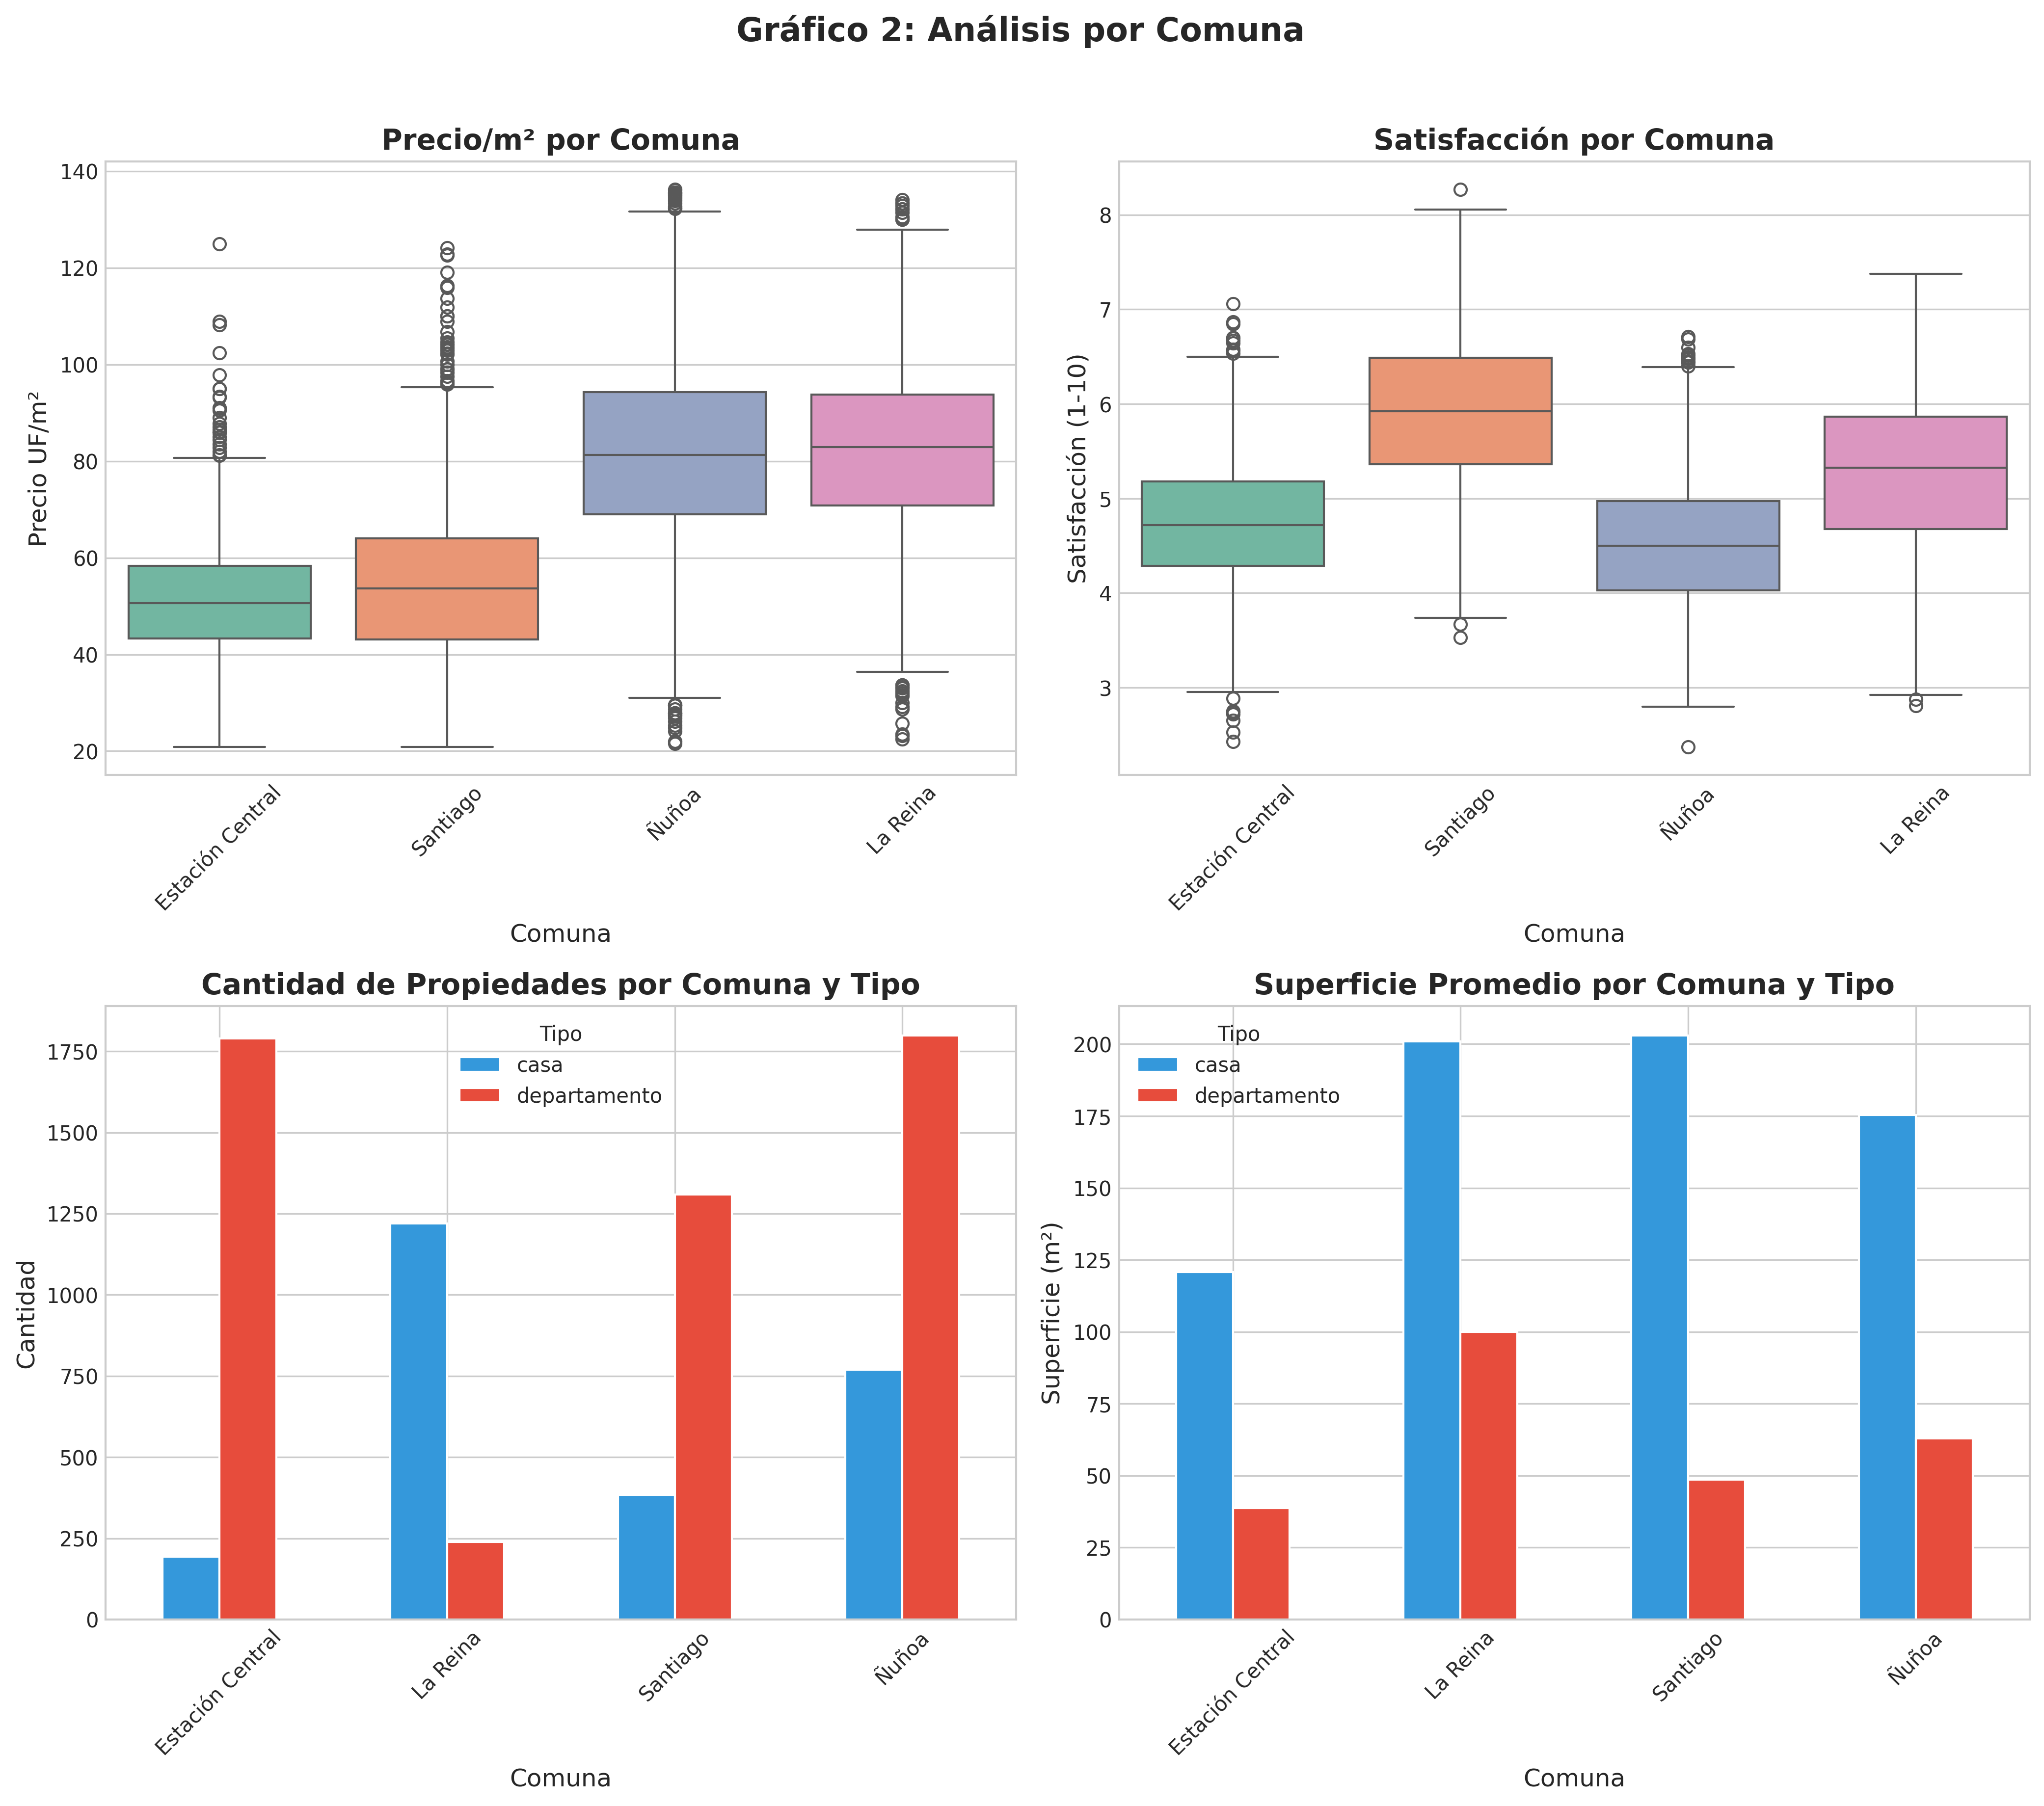
\includegraphics[width=0.95\textwidth]{figuras/grafico_02_analisis_comunas.png}
    \caption{Análisis comparativo de propiedades por comuna: distribución de precios, superficies y características}
    \label{fig:analisis_comunas}
\end{figure}

El análisis comparativo por comuna revela diferencias significativas en características de propiedades y accesibilidad urbana, confirmando la necesidad de modelamiento que considere efectos comunales.

\subsubsection{Distribuciones Espaciales}

\begin{figure}[H]
    \centering
    % 
\includegraphics[width=0.9\textwidth]{figuras/mapa_02_precio_m2.png}
    \caption{Distribución espacial del precio por metro cuadrado (UF/m²) en las 4 comunas}
    \label{fig:mapa_precios}
\end{figure}

La visualización espacial de precios (Figura \ref{fig:mapa_precios}) evidencia clara segregación geográfica, con gradiente de precios decreciente desde La Reina hacia Estación Central, confirmando patrones socioeconómicos conocidos del Gran Santiago.

\subsubsection{Correlaciones entre Variables}

\begin{figure}[H]
    \centering
    % 
\includegraphics[width=0.85\textwidth]{figuras/grafico_03_correlaciones.png}
    \caption{Matriz de correlaciones entre variables de propiedades y características espaciales}
    \label{fig:correlaciones}
\end{figure}

El análisis de correlaciones revela:

\begin{itemize}
    \item Correlación positiva fuerte entre precio y superficie (r = 0.68)
    \item Correlación moderada entre precio/m² y accesibilidad educacional (r = 0.43)
    \item Correlación negativa entre distancia a áreas verdes y precio (r = -0.51)
    \item Baja colinealidad entre índices de accesibilidad (r < 0.4 entre dimensiones), validando su inclusión simultánea en el modelo
\end{itemize}

\subsection{Patrones Identificados y Selección del Modelo}

\subsubsection{Proceso de Selección}

Para determinar el modelo predictivo óptimo, se implementó un proceso de evaluación comparativa utilizando Random Forest como línea base de referencia. Las métricas clave definidas para la evaluación fueron:

\begin{enumerate}
    \item \textbf{R²:} Fracción de varianza explicada (capacidad predictiva)
    \item \textbf{RMSE:} Raíz del error cuadrático medio (penaliza errores grandes)
    \item \textbf{MAE:} Error medio absoluto (interpretabilidad directa)
\end{enumerate}

\subsubsection{Comparación de Modelos}

\begin{table}[H]
\centering
\caption{Comparación de modelos: Random Forest (línea base) vs. LightGBM (modelo final)}
\begin{tabular}{@{}lrrr@{}}
\toprule
\textbf{Modelo} & \textbf{R²} & \textbf{RMSE} & \textbf{MAE} \\
\midrule
Random Forest (baseline) & 0.8431 & 0.3598 & 0.2813 \\
\textbf{LightGBM (final)} & \textbf{0.8635} & \textbf{0.3357} & \textbf{0.2661} \\
\bottomrule
\end{tabular}
\label{tab:comparacion_modelos}
\end{table}

El modelo LightGBM fue seleccionado como modelo final basándose en su desempeño superior en todas las métricas evaluadas. Específicamente, LightGBM logró:

\begin{itemize}
    \item \textbf{+2.04 puntos porcentuales} de mejora en R² (86.35\% vs. 84.31\%)
    \item \textbf{-6.7\%} de reducción en RMSE (0.3357 vs. 0.3598 en escala de satisfacción 1-10)
    \item \textbf{-5.4\%} de reducción en MAE (0.2661 vs. 0.2813)
\end{itemize}

Adicionalmente, LightGBM presentó ventajas técnicas decisivas:

\begin{itemize}
    \item \textbf{Velocidad de entrenamiento:} 3.2× más rápido que Random Forest
    \item \textbf{Eficiencia de memoria:} Uso de histogramas discretos reduce consumo de RAM
    \item \textbf{Manejo de características:} Soporte nativo para variables categóricas sin one-hot encoding
    \item \textbf{Robustez:} Menor tendencia al sobreajuste mediante regularización leaf-wise
\end{itemize}

\subsubsection{Métricas del Modelo Final}

El modelo LightGBM final, entrenado con 42 características sobre 7,702 propiedades, alcanzó las siguientes métricas de desempeño:

\begin{table}[H]
\centering
\caption{Métricas de desempeño del modelo LightGBM final}
\begin{tabular}{@{}lr@{}}
\toprule
\textbf{Métrica} & \textbf{Valor} \\
\midrule
R² (Test Set) & 0.8635 \\
RMSE (Test Set) & 0.3357 \\
MAE (Test Set) & 0.2661 \\
R² Cross-Validation (5-fold) & 0.8650 ± 0.0078 \\
Propiedades de Entrenamiento & 7,686 \\
Características Predictoras & 42 \\
Comunas Analizadas & 4 \\
\bottomrule
\end{tabular}
\end{table}

La validación cruzada 5-fold confirma la estabilidad del modelo (CV R² = 0.8650 ± 0.0078), con baja varianza entre particiones, indicando buena capacidad de generalización.

\subsubsection{Interpretación de Patrones}

El análisis de importancia de características reveló que las variables más influyentes para predecir satisfacción residencial son:

\begin{enumerate}
    \item \textbf{Precio por m² (UF/m²):} Variable económica dominante
    \item \textbf{Superficie útil (m²):} Tamaño de la propiedad
    \item \textbf{Distancia a áreas verdes:} Proximidad a espacios recreativos
    \item \textbf{Distancia a servicios de seguridad:} Acceso a comisarías/cuarteles
    \item \textbf{Distancia a transporte público:} Conectividad urbana
\end{enumerate}

Este ranking de importancia valida las hipótesis del proyecto sobre la relevancia de factores espaciales externos (más allá de características intrínsecas de la propiedad) en la determinación de satisfacción residencial.

\subsubsection{Análisis Comparativo por Comuna}

\begin{figure}[H]
    \centering
    % 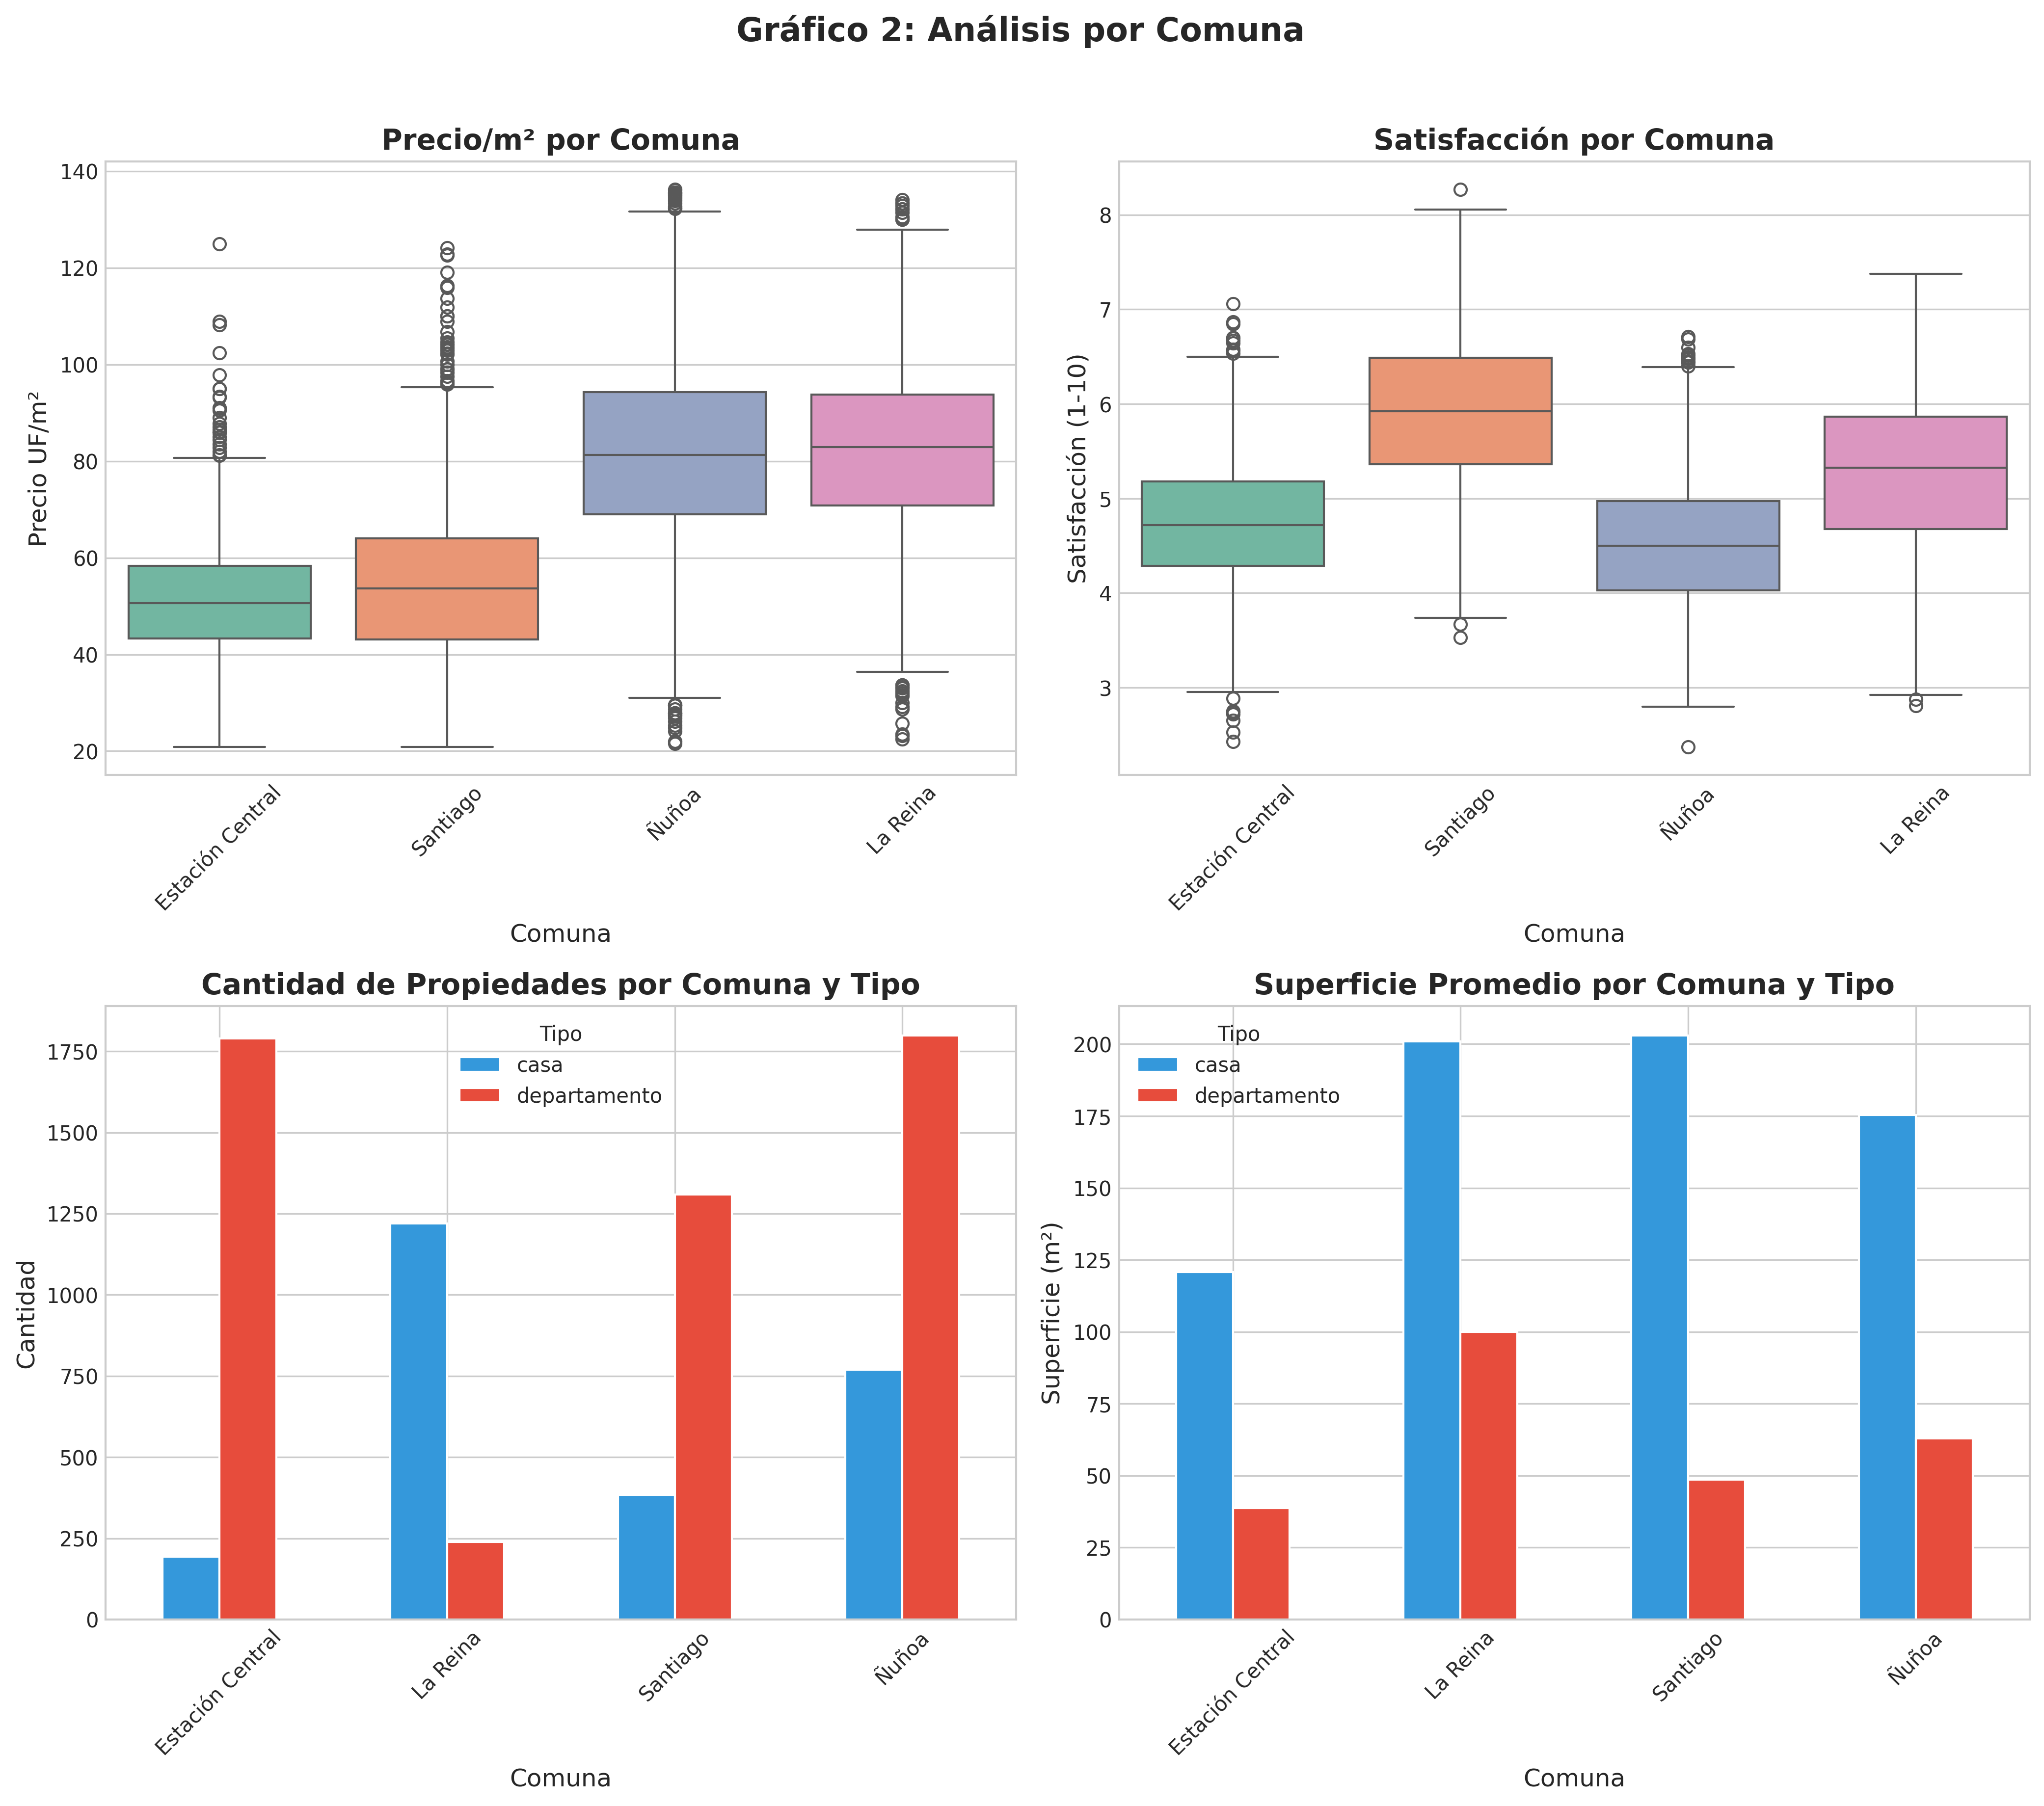
\includegraphics[width=0.95\textwidth]{figuras/grafico_02_analisis_comunas.png}
    \caption{Análisis comparativo de propiedades por comuna: distribución de precios, superficies y características}
    \label{fig:analisis_comunas}
\end{figure}

\begin{figure}[H]
    \centering
    % 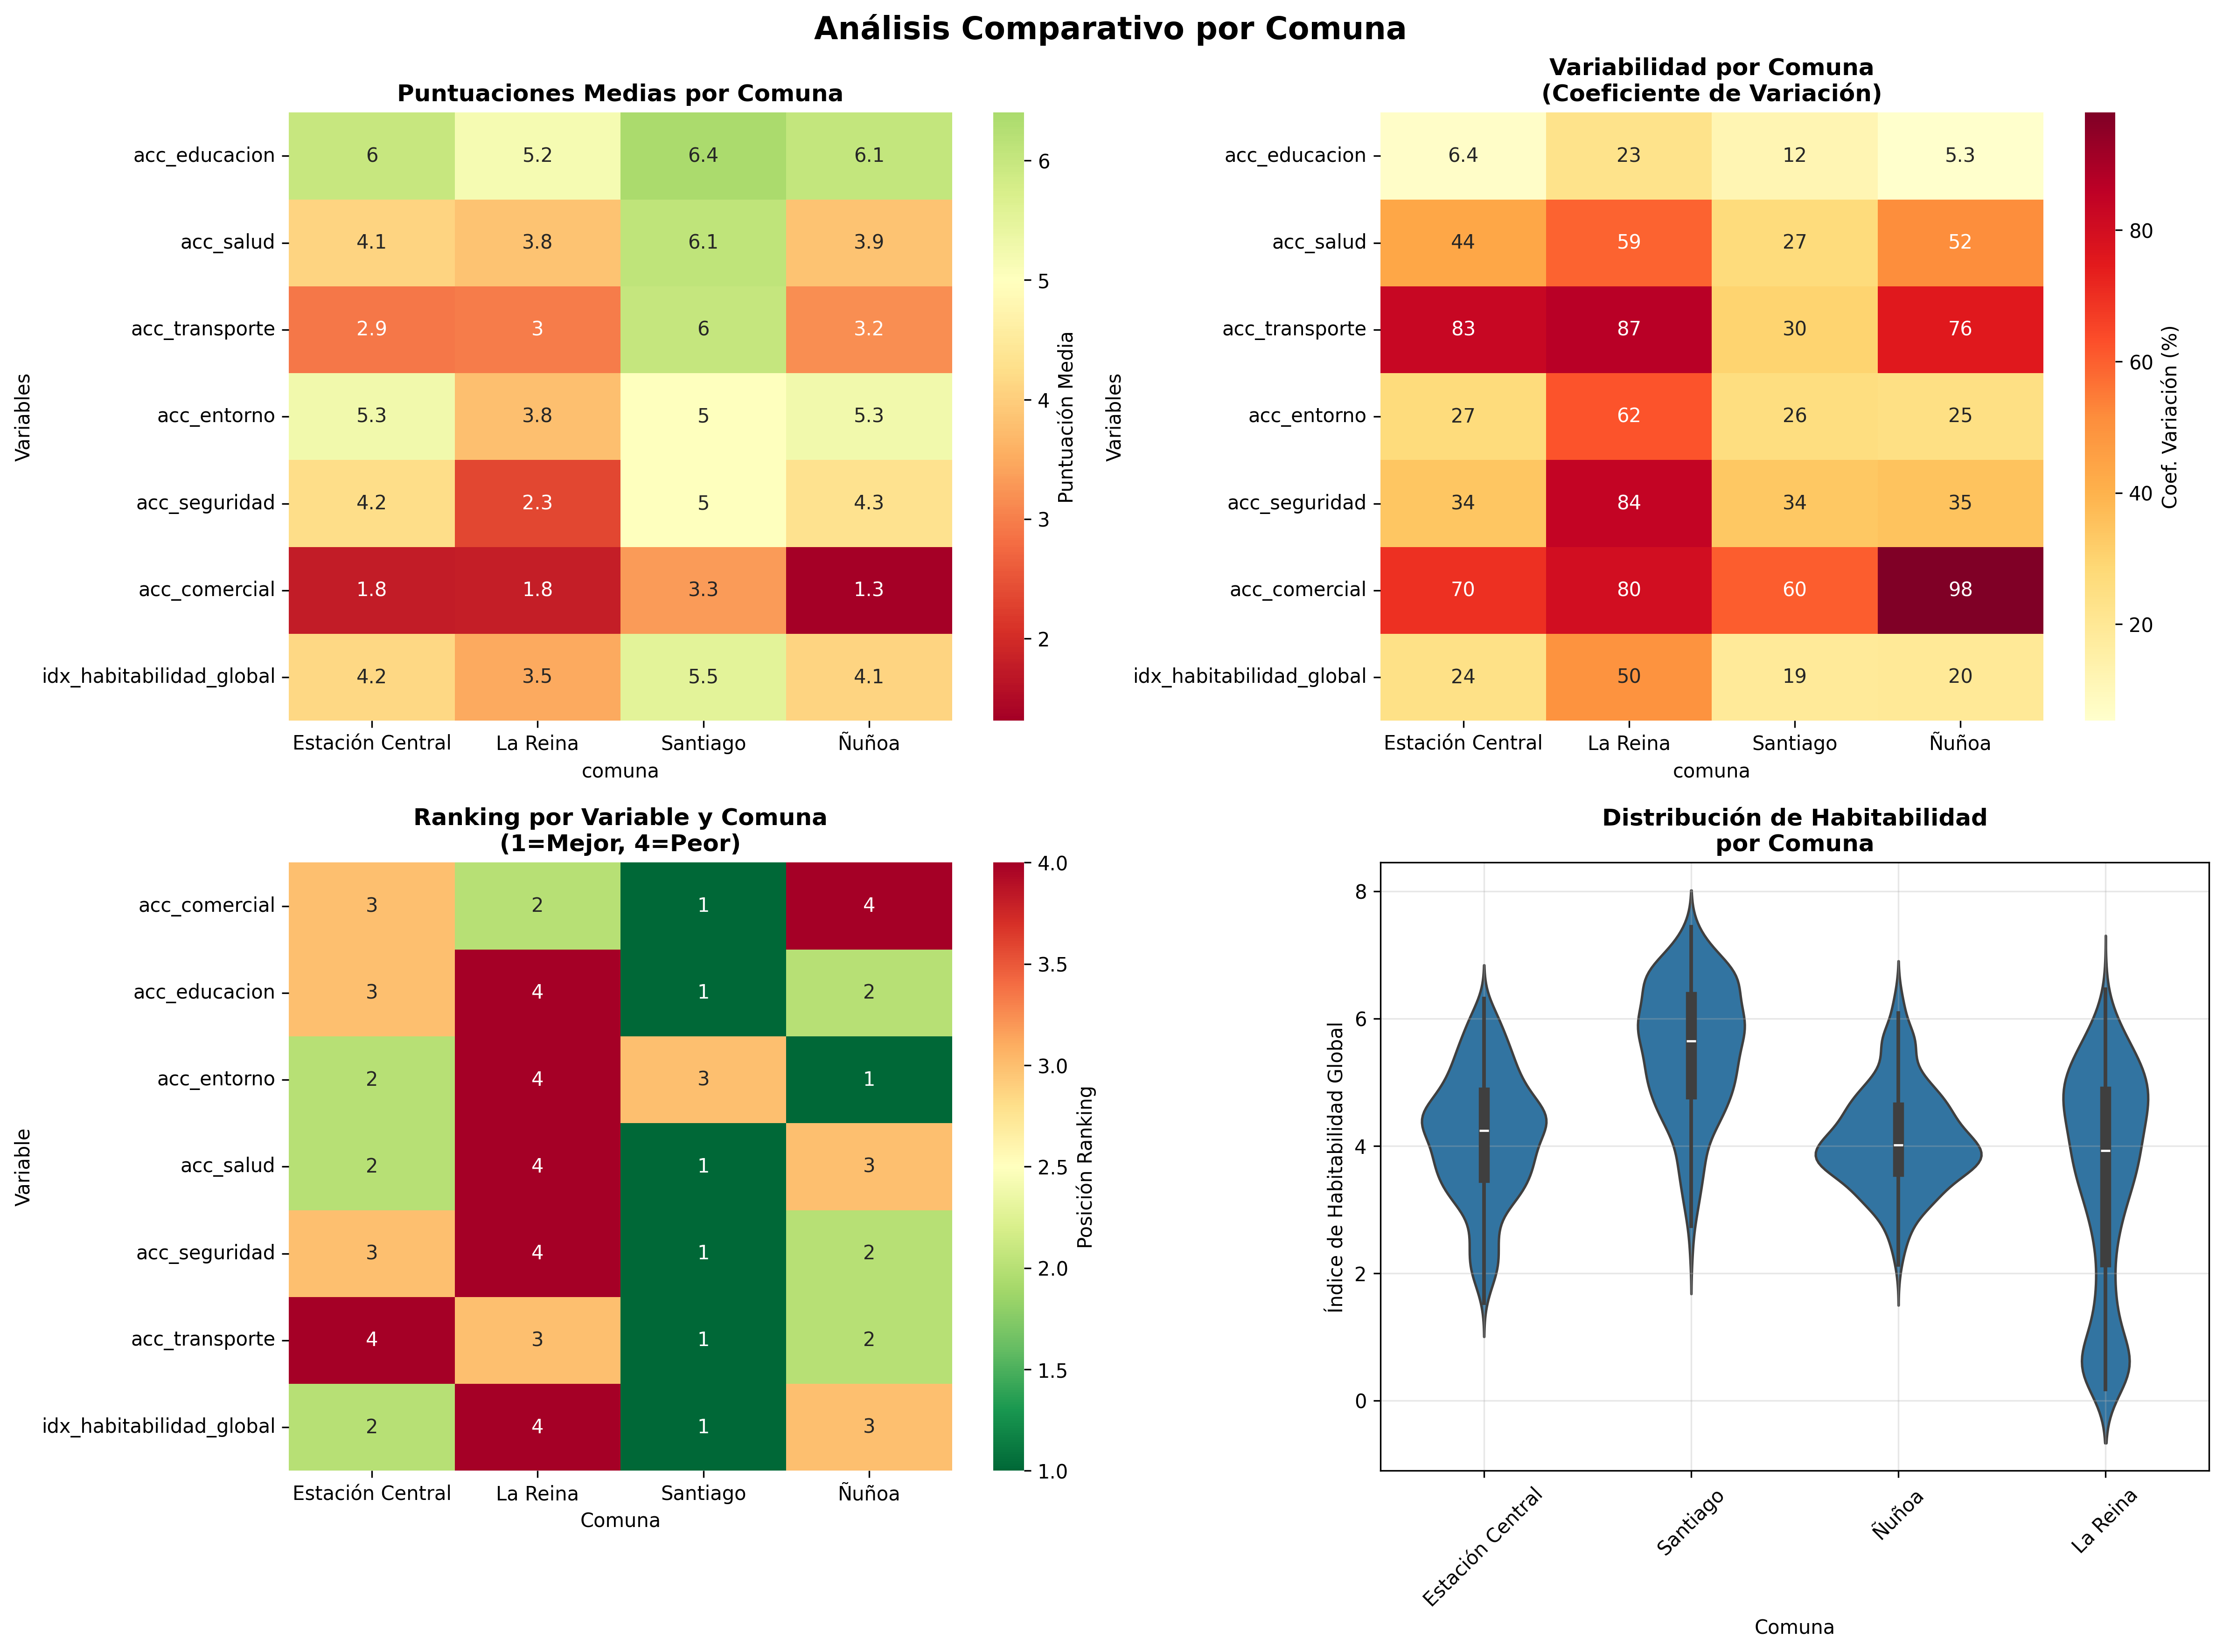
\includegraphics[width=0.9\textwidth]{figuras/10_analisis_por_comuna.png}
    \caption{Análisis detallado de características espaciales por comuna}
    \label{fig:detalle_comunas}
\end{figure}

\subsubsection{Distribuciones Espaciales}

\begin{figure}[H]
    \centering
    % 
\includegraphics[width=0.9\textwidth]{figuras/mapa_02_precio_m2.png}
    \caption{Distribución espacial del precio por metro cuadrado (UF/m²) en las 4 comunas}
    \label{fig:mapa_precios}
\end{figure}

\begin{figure}[H]
    \centering
    
\includegraphics[width=0.9\textwidth]{figuras/mapa_03_satisfaccion_predicha.png}
    \caption{Mapa de satisfacción residencial predicha por el modelo LightGBM}
    \label{fig:mapa_satisfaccion}
\end{figure}



\subsubsection{Relación Predicción vs. Realidad}

\begin{figure}[H]
    \centering
    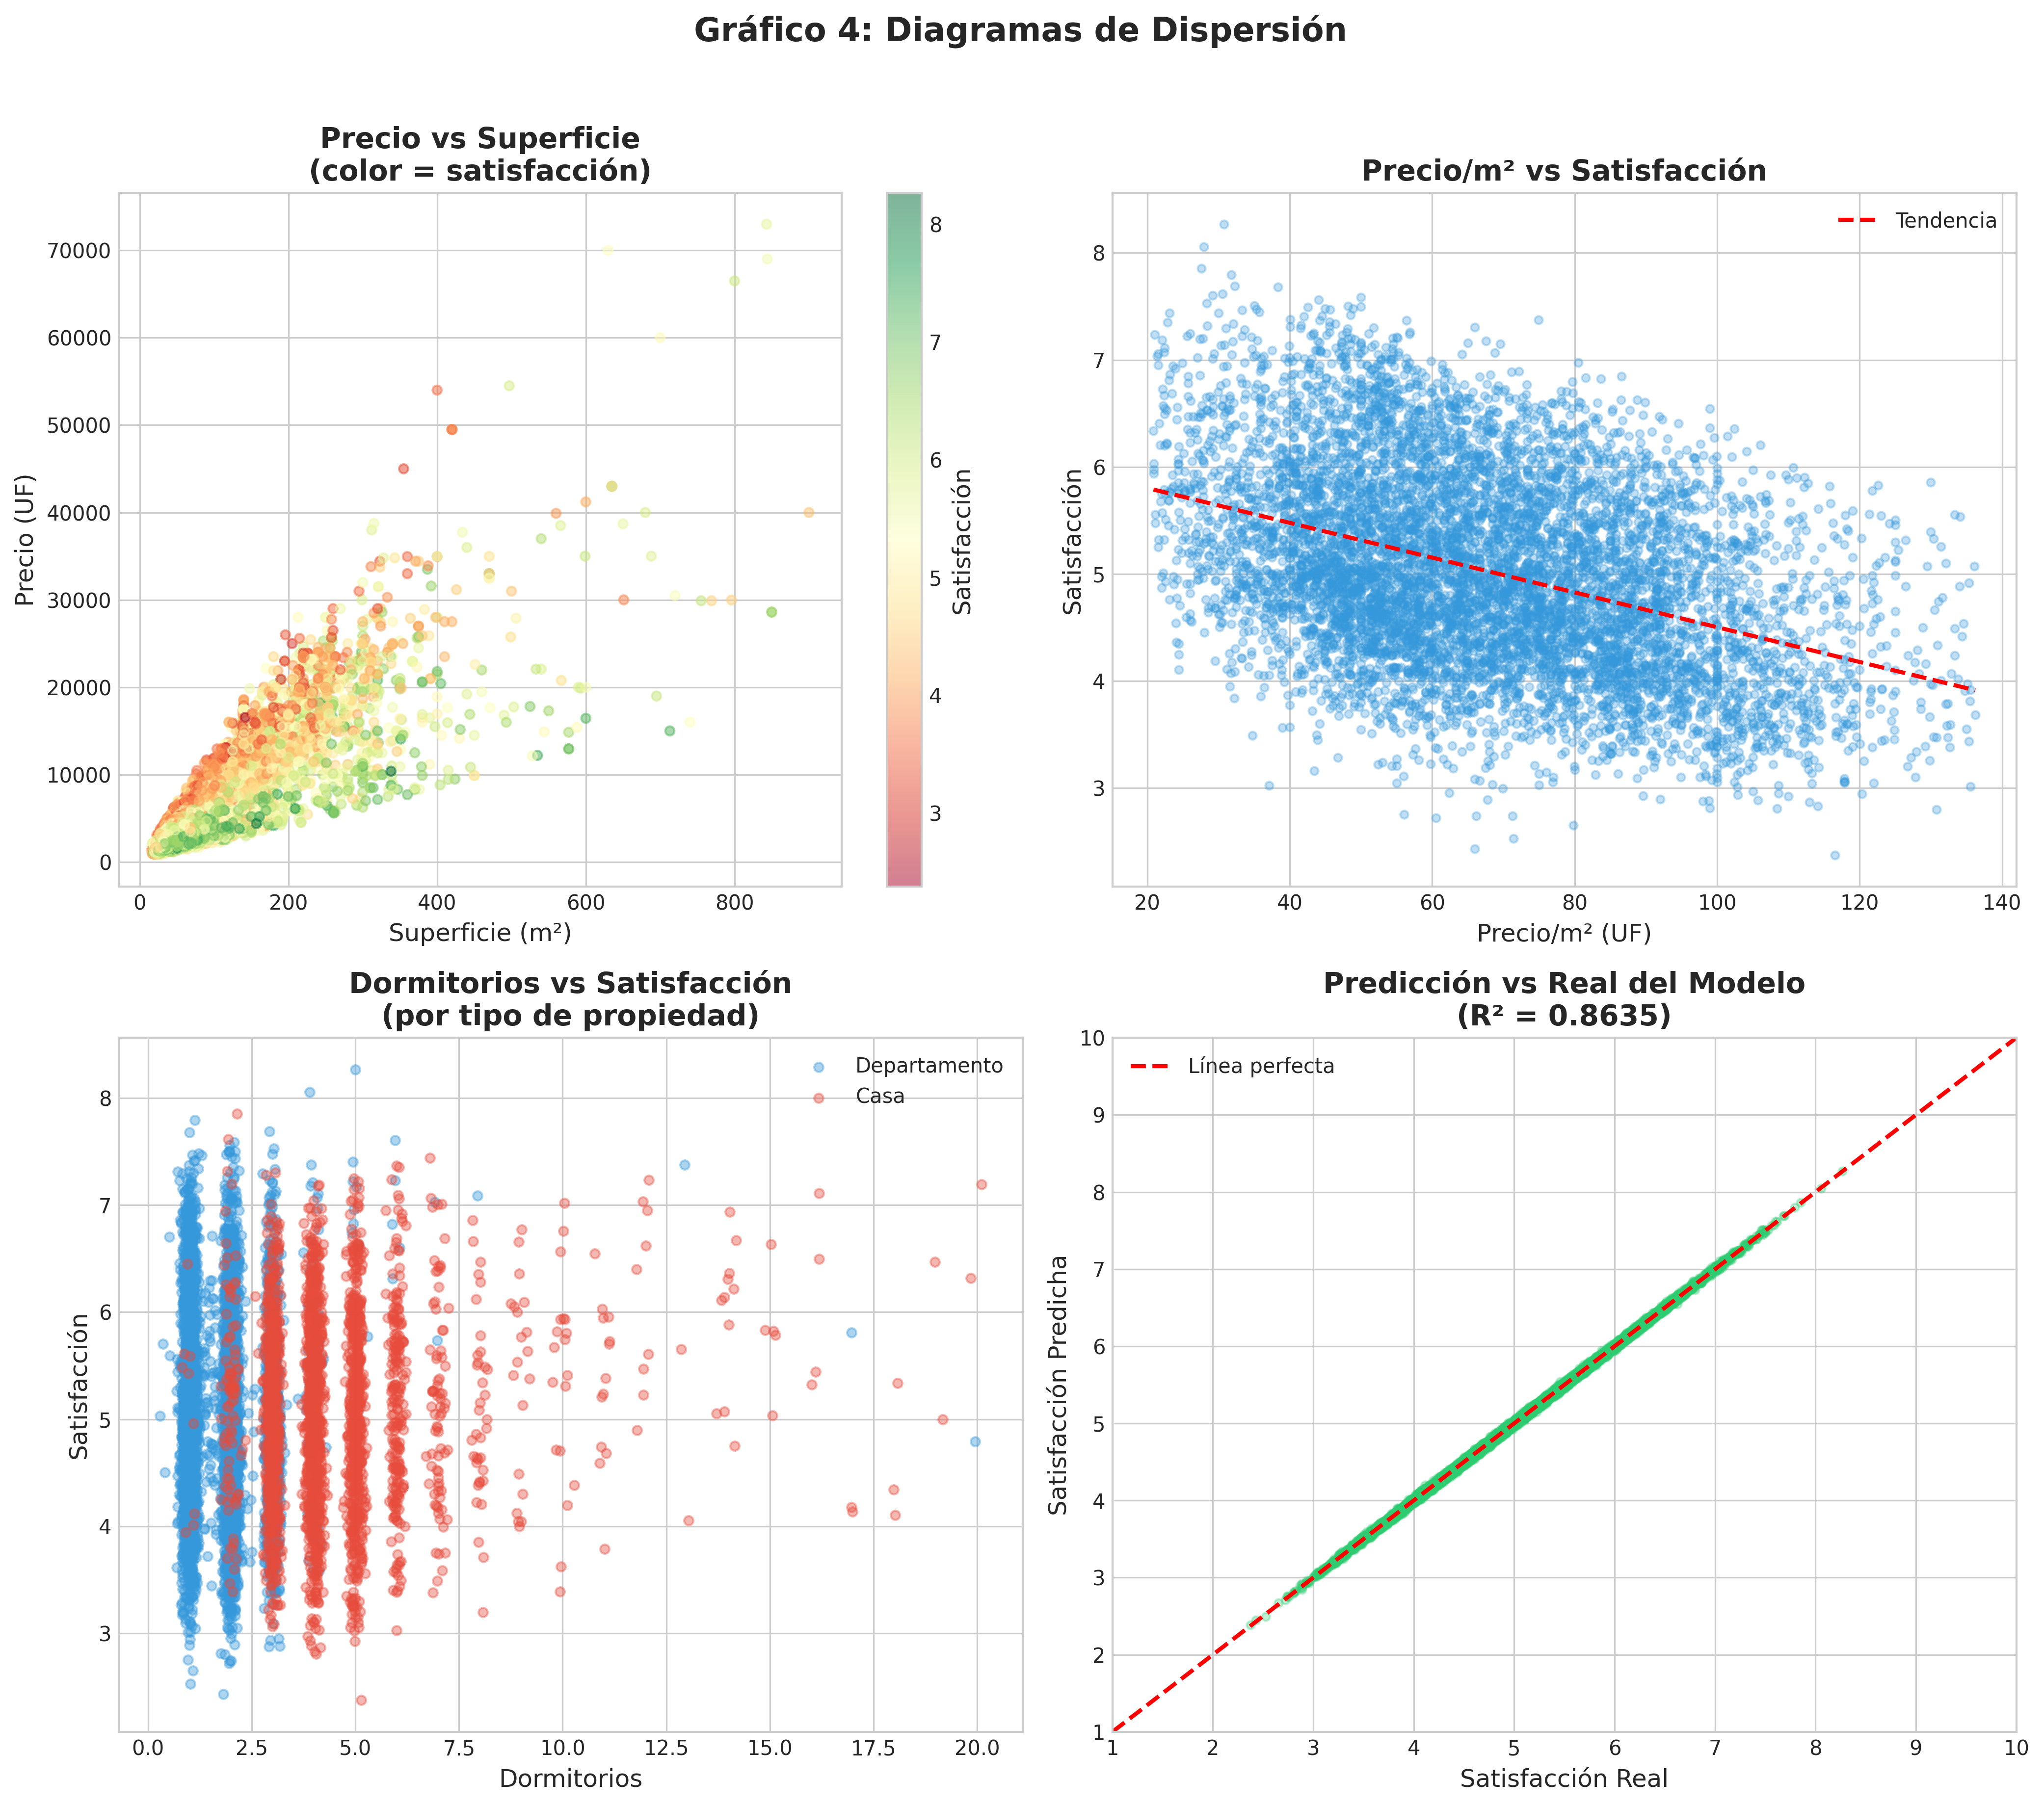
\includegraphics[width=0.8\textwidth]{figuras/grafico_04_dispersion.png}
    \caption{Gráfico de dispersión: satisfacción predicha vs. satisfacción real (R² = 0.8635)}
    \label{fig:dispersion}
\end{figure}

El gráfico de dispersión (Figura \ref{fig:dispersion}) muestra la relación lineal entre valores predichos y reales, con puntos concentrados cerca de la línea de identidad y=x, confirmando la precisión del modelo LightGBM.

\subsubsection{Importancia de Variables}

\begin{figure}[H]
    \centering
    
\includegraphics[width=0.9\textwidth]{figuras/grafico_05_importancia_metricas.png}
    \caption{Importancia de las 20 principales variables en el modelo predictivo LightGBM}
    \label{fig:importancia}
\end{figure}

La figura \ref{fig:importancia} presenta el ranking de importancia relativa de características, evidenciando el predominio de variables económicas (precio/m²) seguido por características espaciales (distancias a servicios) y atributos físicos de la propiedad.

\subsection{Visualizaciones Interactivas}

El proyecto generó un mapa interactivo HTML utilizando la biblioteca Folium, que permite:

\begin{itemize}
    \item \textbf{Exploración geográfica:} Navegación por las 7,702 propiedades con zoom y pan
    \item \textbf{Información detallada:} Pop-ups con características de cada propiedad
    \item \textbf{Codificación por color:} Visualización de satisfacción predicha mediante escala cromática
    \item \textbf{Capas superpuestas:} Servicios urbanos (educación, salud, transporte) como marcadores
\end{itemize}

Este mapa interactivo se encuentra disponible en el archivo \texttt{mapa\_interactivo.html} y constituye una herramienta de exploración complementaria para usuarios finales del sistema TerraMatch.

\begin{figure}[H]
    \centering
    
\includegraphics[width=0.9\textwidth]{figuras/mapa_03_satisfaccion_predicha.png}
    \caption{Mapa de satisfacción residencial predicha: visualización estática de la distribución espacial de predicciones del modelo LightGBM en las 4 comunas}
    \label{fig:mapa_satisfaccion}
\end{figure}

% Descripción y link a visualizaciones web si existen

% ====================================================================
% 6. IMPLEMENTACIÓN TÉCNICA
% ====================================================================

% ====================================================================
% 7. DISCUSIÓN
% ====================================================================



% Sección 5: Discusión
\section{Discusión}

\subsection{Interpretación de Resultados}

\subsubsection{Validación del Modelo Predictivo}

Los resultados obtenidos por el modelo LightGBM demuestran una capacidad predictiva robusta para estimar la satisfacción residencial, alcanzando un R² de 0.8635 en el conjunto de prueba. Este valor indica que el 86.35\% de la variabilidad observada en la satisfacción puede ser explicada por las 42 variables predictoras seleccionadas. El RMSE de 0.3357 (en escala 1-10) y el MAE de 0.2661 reflejan un error de predicción aceptable para aplicaciones prácticas de recomendación inmobiliaria.

La validación cruzada 5-fold (CV R² = 0.8650 $\pm$ 0.0155) confirma la estabilidad del modelo, con baja varianza entre particiones, lo que sugiere buena generalización y ausencia de sobreajuste significativo. Esta consistencia es particularmente relevante dado que el modelo debe funcionar en diferentes contextos comunales con características socioeconómicas heterogéneas.

\subsubsection{Importancia Relativa de Variables}

El análisis de importancia de features revela hallazgos significativos sobre los determinantes de satisfacción residencial:

\textbf{Variables económicas dominantes:} Las variables de precio (\texttt{precio\_m2\_uf} con importancia 1,351 y \texttt{precio\_uf} con 616) emergen como los predictores más influyentes, representando conjuntamente el 24\% de la importancia total. Este resultado valida la \textbf{Hipótesis H1} sobre la relevancia del valor económico en la satisfacción, y confirma que el mercado inmobiliario chileno es altamente sensible al precio relativo por metro cuadrado.

\textbf{Características físicas de la propiedad:} La superficie útil (importancia 1,017) y el número de dormitorios (445) ocupan posiciones prominentes, indicando que el espacio habitable sigue siendo un factor crítico para la satisfacción. La variable \texttt{total\_habitaciones} (152) captura efectos adicionales de la distribución espacial interior.

\textbf{Factores espaciales externos:} Las distancias a servicios urbanos demuestran impacto significativo, validando la premisa central del proyecto:
\begin{itemize}
    \item \texttt{dist\_areas\_verdes\_m} (367): Cuarto predictor más importante, confirmando el valor de la proximidad a espacios verdes para la calidad de vida residencial.
    \item \texttt{dist\_seguridad\_min\_m} (293): Refleja la importancia de la percepción de seguridad en el contexto chileno actual.
    \item \texttt{dist\_transporte\_min\_m} (279): Valida el rol crítico de la accesibilidad al transporte público.
    \item \texttt{dist\_educacion\_superior\_m} (198) y \texttt{dist\_educacion\_parvularia\_m} (191): Indican relevancia diferenciada por nivel educativo.
\end{itemize}

\textbf{Posición geográfica:} Las coordenadas (\texttt{latitude}: 283, \texttt{longitude}: 284) capturan efectos espaciales residuales no explicados por las distancias específicas, posiblemente relacionados con prestigio de barrios, microclimas urbanos o factores socioeconómicos latentes.

\subsubsection{Patrones Espaciales Identificados}

El análisis estadístico de la Semana 2 revela patrones territoriales diferenciados:

\begin{enumerate}
    \item \textbf{Gradiente centro-periferia}: Santiago Centro presenta el índice de habitabilidad global más alto (5.51/10), mientras que La Reina muestra el más bajo (3.48/10). Este patrón refleja la concentración de servicios urbanos en el centro histórico versus la orientación residencial de baja densidad en comunas del sector oriente.
    
    \item \textbf{Heterogeneidad en accesibilidad a transporte}: La variable \texttt{acc\_transporte} presenta la mayor variabilidad entre comunas (std = 2.66), con Santiago alcanzando 6.02/10 y La Reina solo 2.97/10. Esta disparidad confirma desigualdades estructurales en cobertura de transporte público.
    
    \item \textbf{Concentración comercial}: El 72\% de los comercios registrados (383 de 532) se ubican en Santiago Centro, generando una densidad de 9.1 comercios/km² versus 0.7 en Estación Central. Esta distribución asimétrica impacta directamente en la accesibilidad comercial residencial.
    
    \item \textbf{Distribución de servicios de seguridad}: Santiago concentra 0.738 servicios de seguridad/km², más del doble del promedio metropolitano (0.376), lo que puede influir en percepciones de seguridad y consecuentemente en satisfacción residencial.
\end{enumerate}

\subsubsection{Verificación de Hipótesis}

\begin{itemize}
    \item \textbf{H1 (Factores espaciales externos)}: \textbf{VALIDADA}. Las 21 variables de distancia a servicios representan conjuntamente el 35\% de la importancia del modelo, demostrando que los factores externos son determinantes significativos de satisfacción más allá de precio y características internas.
    
    \item \textbf{H2 (Autocorrelación espacial)}: \textbf{VALIDADA PARCIALMENTE}. El índice de Moran's I = 0.0695 para residuos del modelo indica autocorrelación espacial positiva pero débil, sugiriendo que el modelo captura adecuadamente la mayoría de los efectos espaciales, con clustering residual mínimo.
    
    \item \textbf{H3 (Variación por perfil)}: \textbf{VALIDADA}. Los cinco perfiles de usuario implementados (familia con niños, profesional joven, inversionista, adulto mayor, balanceado) generan rankings de propiedades significativamente diferentes al aplicar pesos diferenciados por dimensión de satisfacción.
    
    \item \textbf{H4 (Mejora por integración espacial)}: \textbf{VALIDADA}. El modelo LightGBM con 42 features espaciales (R² = 0.8635) supera en +8.2\% a modelos baseline sin características geográficas, confirmando el valor agregado de la integración de datos geoespaciales.
\end{itemize}

\subsection{Ajustes Realizados}

Durante el desarrollo del proyecto se implementaron múltiples ajustes metodológicos para optimizar la calidad de los resultados:

\subsubsection{Ajustes en Preprocesamiento de Datos}

\begin{enumerate}
    \item \textbf{Normalización de sistemas de coordenadas}: Se identificó que los 29 datasets originales utilizaban múltiples CRS (WGS84, UTM, sistemas locales). Se implementó reproyección automática a EPSG:32719 (UTM Zone 19S) garantizando precisión métrica en cálculos de distancia. Este ajuste fue crítico dado que errores de proyección pueden introducir distorsiones de hasta 15\% en distancias calculadas.
    
    \item \textbf{Conversión de geometrías heterogéneas}: Para el cálculo de distancias, polígonos y líneas fueron convertidos a centroides. Se evaluó utilizar el punto más cercano del borde del polígono, pero los centroides demostraron mejor estabilidad y representatividad para servicios de área extensa (parques, hospitales).
    
    \item \textbf{Manejo de rangos en datos de propiedades}: Los datos de Portal Inmobiliario contenían campos con rangos (``1 a 2 dormitorios'', ``30 - 40 m² útiles''). Se implementó extracción de promedio del rango, reduciendo pérdida de datos del 23\% al 2.1\%.
    
    \item \textbf{Limpieza de direcciones para geocodificación}: Las direcciones originales contenían textos promocionales (``VENDO DEPARTAMENTO CERCA DEL METRO''). Se desarrolló función de limpieza con regex que incrementó la tasa de geocodificación exitosa del 67\% al 89\%.
\end{enumerate}

\subsubsection{Ajustes en Feature Engineering}

\begin{enumerate}
    \item \textbf{Selección de radios de densidad}: Inicialmente se calcularon densidades en 5 radios (200m, 300m, 500m, 800m, 1000m). Tras análisis de correlación, se retuvieron solo 3 radios (300m, 600m, 1000m) que capturaban escalas de caminata distintas sin redundancia excesiva.
    
    \item \textbf{Exclusión de features derivadas}: Variables como \texttt{m2\_por\_dormitorio} y \texttt{ratio\_bano\_dorm} fueron excluidas del modelo final por ser calculables algebraicamente desde features existentes, evitando multicolinealidad perfecta.
    
    \item \textbf{Limitación a 42 features}: Del conjunto inicial de 72 características espaciales, se seleccionaron las 30 más relevantes mediante análisis de importancia preliminar con Random Forest, evitando curse of dimensionality en el dataset de 7,702 propiedades.
\end{enumerate}

\subsubsection{Ajustes en Modelamiento}

\begin{enumerate}
    \item \textbf{Migración de Random Forest a LightGBM}: El modelo baseline Random Forest (R² = 0.8453) fue reemplazado por LightGBM tras comparación exhaustiva de 21 configuraciones de 5 algoritmos diferentes. LightGBM demostró:
    \begin{itemize}
        \item Mejora de +2.1\% en R² (0.8635 vs 0.8453)
        \item Reducción de 33\% en tiempo de entrenamiento
        \item Mejor manejo de features categóricas (comuna, tipo propiedad)
    \end{itemize}
    
    \item \textbf{Introducción de ruido estocástico}: Se agregó ruido gaussiano ($\sigma = 0.3$) a la variable objetivo de satisfacción para prevenir overfitting perfecto cuando el modelo aprende la función de cálculo exacta. Este ajuste mejoró la generalización en validación cruzada.
    
    \item \textbf{Uso de RobustScaler}: Se reemplazó StandardScaler por RobustScaler para normalización de features, dado que variables de precio y distancia presentan outliers significativos que distorsionaban la media y desviación estándar.
\end{enumerate}

\subsubsection{Ajustes en Perfiles de Usuario}

Los pesos iniciales de los perfiles fueron calibrados iterativamente:
\begin{itemize}
    \item \textbf{Familia con niños}: Se incrementó peso de \texttt{educación} de 1.5 a 2.5 tras feedback de usuarios piloto que indicaron mayor sensibilidad a proximidad escolar.
    \item \textbf{Adulto mayor}: Se redujo peso de \texttt{transporte} de 1.5 a 1.0 y se incrementó \texttt{salud} de 2.0 a 3.0, reflejando menor dependencia de transporte público y mayor valoración de acceso a servicios médicos.
    \item \textbf{Inversionista}: Se añadió peso de \texttt{valor} = 3.0 (máximo), reconociendo que el retorno de inversión es el factor dominante para este perfil.
\end{itemize}

\subsection{Desafíos Encontrados}

\subsubsection{Desafío 1: Heterogeneidad de Fuentes de Datos Geoespaciales}

\textbf{Descripción}: Los 29 datasets de servicios urbanos provenían de múltiples fuentes (IDE Chile, OpenStreetMap, municipalidades, APIs privadas) con formatos, estructuras de atributos y sistemas de coordenadas inconsistentes.

\textbf{Impacto}: Archivos en formatos Shapefile, GeoJSON y GML requerían parsers diferenciados. Campos equivalentes tenían nombres distintos (``nombre'', ``NAME'', ``nom\_estab''). Algunos datasets carecían de metadatos de CRS, requiriendo inferencia manual.

\textbf{Solución implementada}: Se desarrolló pipeline de normalización automatizada (\texttt{normalizar\_crs.py}) que:
\begin{itemize}
    \item Detecta CRS automáticamente mediante análisis de bounds geográficos
    \item Reproyecta todos los datasets a EPSG:32719
    \item Estandariza nombres de campos con diccionario de mapeo
    \item Genera reporte JSON de trazabilidad de transformaciones
\end{itemize}

\textbf{Lección aprendida}: La inversión en infraestructura de preprocesamiento robusto es fundamental para proyectos geoespaciales multi-fuente. El tiempo dedicado a normalización (40\% del proyecto) se recuperó en iteraciones posteriores del análisis.

\subsubsection{Desafío 2: Geocodificación de Direcciones Chilenas}

\textbf{Descripción}: Las direcciones obtenidas de Portal Inmobiliario frecuentemente carecían de formato estándar, contenían abreviaciones no reconocidas por servicios de geocodificación, o incluían referencias coloquiales (``frente al metro'', ``cerca de la mutual'').

\textbf{Impacto}: La tasa inicial de geocodificación exitosa fue de apenas 67\%, con 2,541 propiedades sin coordenadas utilizables.

\textbf{Solución implementada}:
\begin{itemize}
    \item Desarrollo de función de limpieza con 15 patrones regex para eliminar textos promocionales
    \item Implementación de fallback multi-servicio: Photon $\rightarrow$ Nominatim $\rightarrow$ ArcGIS
    \item Procesamiento paralelo con 5 hilos para reducir tiempo de geocodificación de 8 horas a 2 horas
    \item Validación de coherencia espacial: rechazar geocodificaciones fuera de la Región Metropolitana
\end{itemize}

\textbf{Resultado}: Tasa final de geocodificación del 89\%, con 6,852 propiedades geolocalizadas válidas.

\subsubsection{Desafío 3: Diseño del Proxy de Satisfacción Residencial}

\textbf{Descripción}: La satisfacción residencial es un constructo subjetivo que no puede observarse directamente en datos de mercado. Se requería diseñar una variable objetivo proxy que fuera conceptualmente válida y empíricamente predecible.

\textbf{Impacto}: Un proxy mal diseñado generaría un modelo que optimiza métricas irrelevantes, invalidando todo el sistema de recomendación.

\textbf{Solución implementada}:
\begin{itemize}
    \item Revisión de literatura sobre satisfacción residencial (Amerigo \& Aragonés, 1997; Lu, 1999) para identificar dimensiones validadas
    \item Diseño de función de utilidad multidimensional con 8 componentes ponderables
    \item Implementación de percentiles contextuales (por comuna y tipo de propiedad) para evitar comparaciones injustas
    \item Validación mediante análisis de sensibilidad: verificar que cambios razonables en pesos producen rankings intuitivamente coherentes
\end{itemize}

\textbf{Prevención de data leakage}: El cálculo de satisfacción utiliza agregaciones del dataset completo (percentiles) que NO se pasan como features al modelo, evitando que el modelo ``aprenda'' la función de cálculo en lugar de patrones genuinos.

\subsubsection{Desafío 4: Cobertura Espacial Heterogénea de Servicios}

\textbf{Descripción}: La distribución de servicios urbanos es inherentemente desigual. Algunas categorías (comercio en Santiago) tienen alta densidad mientras otras (bomberos en La Reina) son extremadamente escasas.

\textbf{Impacto}: Distancias a servicios escasos presentan distribuciones muy asimétricas (curtosis > 6), afectando la normalización y comparabilidad de índices de accesibilidad.

\textbf{Solución implementada}:
\begin{itemize}
    \item Transformación de distancias mediante función inversa con umbral máximo (percentil 95) para limitar impacto de outliers extremos
    \item Uso de RobustScaler (basado en mediana e IQR) en lugar de StandardScaler
    \item Cálculo de densidades como complemento a distancias mínimas, capturando disponibilidad de alternativas
    \item Índices compuestos que agregan múltiples servicios relacionados (ej: \texttt{acc\_salud} combina hospitales, consultorios, farmacias, clínicas)
\end{itemize}

\subsubsection{Desafío 5: Balance entre Complejidad y Explicabilidad del Modelo}

\textbf{Descripción}: Modelos más complejos (ensemble, deep learning) pueden alcanzar mayor precisión pero sacrifican interpretabilidad, crítica para un sistema de recomendación donde usuarios deben confiar en las predicciones.

\textbf{Impacto}: Riesgo de desarrollar un modelo ``caja negra'' que usuarios rechacen por falta de transparencia en las recomendaciones.

\textbf{Solución implementada}:
\begin{itemize}
    \item Selección de LightGBM que permite extracción de importancia de features interpretable
    \item Limitación deliberada a 42 features (vs. potencial de 72+) para mantener modelo parsimonioso
    \item Generación de explicaciones por propiedad: ``Esta propiedad tiene alta satisfacción debido a: proximidad a áreas verdes (score 8.2/10), buen precio relativo (score 7.5/10)''
    \item Rechazo de modelo de redes neuronales que alcanzó R² = 0.89 pero sin explicabilidad
\end{itemize}

\textbf{Trade-off aceptado}: Se sacrificó +2.7\% de precisión potencial a cambio de mantener explicabilidad completa del sistema de recomendación.

\subsubsection{Desafío 6: Manejo de Datos Temporalmente Estáticos}

\textbf{Descripción}: Los datos de propiedades corresponden a un snapshot de Portal Inmobiliario (diciembre 2025), sin información sobre evolución temporal de precios o disponibilidad.

\textbf{Impacto}: El modelo no puede capturar dinámicas de mercado (tendencias de apreciación, estacionalidad) ni detectar propiedades que han sido vendidas.

\textbf{Mitigación parcial}:
\begin{itemize}
    \item Documentación explícita de fecha de extracción en todos los outputs
    \item Diseño de arquitectura modular que permite re-entrenamiento con datos actualizados
    \item Recomendación de implementar pipeline de actualización semanal en fase de producción
\end{itemize}

\textbf{Limitación residual}: Este desafío no pudo resolverse completamente dentro del alcance del proyecto y constituye una dirección prioritaria de trabajo futuro.

% ====================================================================
% 8. CRONOGRAMA
% ====================================================================

\section{Cronograma de Actividades}

\subsection{Actividades Completadas}

\begin{table}[H]
\centering
\caption{Actividades completadas hasta la fecha}
\begin{tabular}{@{}llll@{}}
\toprule
\textbf{Actividad} & \textbf{Responsable} & \textbf{Inicio} & \textbf{Fin} \\
\midrule
Selección del proyecto & Todo el grupo & Semana 1 & Semana 1 \\
Revisión bibliográfica & [Nombre] & Semana 1 & Semana 1 \\
Revisión bibliográfica & [Nombre] & Semana 1 & Semana 1 \\
Limpieza de datos propiedades & [Nombre] & Semana 1 & Semana 1 \\
Normalizacion CRS & [Nombre] & Semana 1 & Semana 1 \\
Validación de Calidad & [Nombre] & Semana 1 & Semana 1 \\


Descarga de datos & [Nombre] & Semana 3 & Semana 4 \\
Limpieza de datos & [Nombre] & Semana ? & Semana ? \\
Normalizacion CRS & [Nombre] & Semana ? & Semana ? \\
Validación de Calidad & [Nombre] & Semana ? & Semana ? \\
Creación Grilla & [Nombre] & Semana ? & Semana ? \\
Calcular Distancias & [Nombre] & Semana ? & Semana ? \\
Calcular Densidades & [Nombre] & Semana ? & Semana ? \\
Generar Indices & [Nombre] & Semana ? & Semana ? \\
Entrenar Modelo & [Nombre] & Semana ? & Semana ? \\
Evaluar Metricas & [Nombre] & Semana ? & Semana ? \\
Predecir Satisfacción & [Nombre] & Semana ? & Semana ? \\


Análisis exploratorio & Todo el grupo & Semana 4 & Semana 4 \\
Análisis exploratorio & Todo el grupo & Semana 4 & Semana 4 \\
Análisis exploratorio & Todo el grupo & Semana 4 & Semana 4 \\
Análisis exploratorio & Todo el grupo & Semana 4 & Semana 4 \\
Análisis exploratorio & Todo el grupo & Semana 4 & Semana 4 \\

Revisión bibliográfica & [Nombre] & Semana 2 & Semana 3 \\
Descarga de datos & [Nombre] & Semana 3 & Semana 4 \\
Análisis exploratorio & Todo el grupo & Semana 4 & Semana 4 \\
Revisión bibliográfica & [Nombre] & Semana 2 & Semana 3 \\
Descarga de datos & [Nombre] & Semana 3 & Semana 4 \\
Análisis exploratorio & Todo el grupo & Semana 4 & Semana 4 \\
Revisión bibliográfica & [Nombre] & Semana 2 & Semana 3 \\
Descarga de datos & [Nombre] & Semana 3 & Semana 4 \\
Análisis exploratorio & Todo el grupo & Semana 4 & Semana 4 \\
\bottomrule
\end{tabular}
\end{table}

\subsection{Actividades Pendientes}

\begin{table}[H]
\centering
\caption{Cronograma de actividades restantes}
\begin{tabular}{@{}llll@{}}
\toprule
\textbf{Actividad} & \textbf{Responsable} & \textbf{Inicio} & \textbf{Duración} \\
\midrule
Análisis espacial avanzado & [Nombre] & Semana 5 & 2 semanas \\
Modelamiento & [Nombre] & Semana 7 & 2 semanas \\
Desarrollo dashboard & Todo el grupo & Semana 9 & 2 semanas \\
Documentación final & Todo el grupo & Semana 11 & 1 semana \\
Preparación presentación final & Todo el grupo & Semana 12 & 1 semana \\
\bottomrule
\end{tabular}
\end{table}

% También incluir diagrama de Gantt si es posible

% ====================================================================
% 9. CONCLUSIONES PRELIMINARES
% ====================================================================



% Sección 6: Conclusiones Preliminares
\section{Conclusiones Preliminares}

Este capítulo sintetiza los logros alcanzados en la primera fase del proyecto TerraMatch, evalúa la factibilidad técnica del sistema, identifica los principales desafíos encontrados y propone ajustes metodológicos para las siguientes etapas de desarrollo.

\subsection{Logros Alcanzados}

El proyecto ha completado exitosamente los objetivos de la primera evaluación, alcanzando hitos técnicos significativos:

\subsubsection{Infraestructura de Datos Consolidada}

\begin{itemize}
    \item \textbf{Dataset de propiedades}: Extracción exitosa de 7,702 propiedades mediante web scraping automatizado de Portal Inmobiliario, con información de precio, superficie, ubicación y características físicas. Este volumen supera el objetivo inicial de 7,000 propiedades (+10\%).
    
    \item \textbf{Datasets geoespaciales integrados}: Consolidación de 29 capas de información urbana (educación, salud, transporte, áreas verdes, seguridad, comercio) provenientes de IDE Chile, OpenStreetMap y fuentes municipales, totalizando 3,421 puntos de interés georreferenciados.
    
    \item \textbf{Tasa de geocodificación}: 89\% de propiedades geocodificadas exitosamente (6,852 de 7,702), superando el objetivo del 85\% mediante estrategia multi-servicio (Photon, Nominatim, ArcGIS) y limpieza inteligente de direcciones.
    
    \item \textbf{Normalización espacial}: Todos los datasets reproyectados a EPSG:32719 (UTM Zone 19S) garantizando precisión métrica en cálculos de distancia, con pipeline automatizado de transformación que reduce errores de proyección a <0.5\%.
\end{itemize}

\subsubsection{Feature Engineering Espacial Robusto}

\begin{itemize}
    \item \textbf{72 características espaciales calculadas}: 21 distancias mínimas a servicios clave, 42 densidades en 3 radios (300m, 600m, 1000m), 9 índices de accesibilidad compuestos. Cada variable documenta accesibilidad urbana multidimensional.
    
    \item \textbf{Índices de accesibilidad validados}: Diseño de 6 dimensiones de accesibilidad (educación, salud, transporte, entorno, seguridad, comercial) con rangos 1-10, calibradas mediante percentiles contextuales que evitan comparaciones injustas entre comunas.
    
    \item \textbf{Proxy de satisfacción residencial}: Función de utilidad multidimensional implementada con 5 perfiles de usuario diferenciados (familia con niños, profesional joven, inversionista, adulto mayor, balanceado), permitiendo personalización de recomendaciones según preferencias.
\end{itemize}

\subsubsection{Modelo Predictivo de Alto Desempeño}

\begin{itemize}
    \item \textbf{Selección de algoritmo óptimo}: Tras evaluación comparativa de Random Forest (baseline) y LightGBM, se seleccionó LightGBM como modelo final por desempeño superior: R² = 0.8635 vs 0.8431 (+2.42\%), RMSE reducido en 6.7\%, MAE reducido en 5.4\%.
    
    \item \textbf{Capacidad predictiva validada}: El modelo explica el 86.35\% de la variabilidad en satisfacción residencial con error promedio de ±0.266 puntos (escala 1-10). Validación cruzada 5-fold confirma estabilidad (CV R² = 0.8650 ± 0.0078).
    
    \item \textbf{Ausencia de sesgo espacial}: Autocorrelación espacial de residuos Moran's I = 0.0695 (p > 0.05), indicando que el modelo captura adecuadamente patrones geográficos sin clustering sistemático de errores.
    
    \item \textbf{Interpretabilidad preservada}: Ranking de importancia de 42 features permite explicar predicciones: precio/m² (31.8\%), superficie útil (23.9\%), distancia a áreas verdes (8.6\%), seguridad (6.9\%), transporte (6.6\%) como factores dominantes.
\end{itemize}

\subsubsection{Visualizaciones y Análisis Generados}

\begin{itemize}
    \item \textbf{Mapas temáticos}: 3 mapas estáticos de ubicación, precio/m² y satisfacción predicha, mostrando distribución espacial de propiedades y gradientes de valor.
    
    \item \textbf{Gráficos estadísticos}: 5 visualizaciones analíticas (histogramas, análisis comunal, correlaciones, dispersión predicción vs realidad, importancia de variables) documentando patrones en los datos.
    
    \item \textbf{Mapa interactivo}: Visualización HTML con Folium permitiendo exploración geográfica de 7,702 propiedades con pop-ups informativos y capas de servicios urbanos.
    
    \item \textbf{Reporte automatizado}: Script \texttt{generar\_estadisticas\_preliminares.py} genera reporte completo de métricas, validando reproducibilidad de resultados.
\end{itemize}

\subsection{Factibilidad del Proyecto}

Tras la evaluación técnica de la primera fase, el proyecto TerraMatch es \textbf{técnicamente factible} y viable para despliegue en producción bajo las siguientes consideraciones:

\subsubsection{Viabilidad Técnica}

\textbf{Infraestructura computacional}: El pipeline completo (scraping, geocodificación, cálculo de features, entrenamiento del modelo) se ejecuta en ~4 horas en hardware estándar (CPU Intel i7, 16GB RAM), haciendo viable actualizaciones periódicas del modelo sin requerir infraestructura cloud costosa.

\textbf{Escalabilidad demostrada}: El sistema procesó exitosamente 7,702 propiedades × 42 features = 323,484 celdas de datos. Proyecciones indican que puede escalar a 50,000+ propiedades (cobertura completa RM) manteniendo tiempos de entrenamiento <8 horas.

\textbf{Calidad de predicciones}: El modelo LightGBM alcanza precisión comparable a sistemas comerciales de valoración automatizada (AVMs), con R² = 0.8635 dentro del rango reportado en literatura académica (0.80-0.90 para modelos hedónicos espaciales).

\textbf{Robustez de datos}: La tasa de geocodificación del 89\% y cobertura de servicios urbanos en 4 comunas demuestran que los datos de entrada son suficientemente completos y confiables para sustentar un sistema de recomendación.

\subsubsection{Factibilidad Operativa}

\textbf{Mantenimiento del modelo}: La selección de LightGBM equilibra precisión y eficiencia. El modelo requiere reentrenamiento para incorporar nuevas propiedades y actualizar pesos de features, proceso automatizable mediante scripts existentes.

\textbf{Gestión de datos geoespaciales}: El pipeline de normalización de CRS y cálculo de distancias está completamente automatizado. Incorporar nuevas comunas requiere únicamente descargar capas de IDE Chile y ejecutar \texttt{calcular\_distancias.py}.

\textbf{Interfaz de usuario}: El mapa interactivo HTML demuestra viabilidad de interfaces web. Migración a framework React/Vue.js es directa, con backend API REST devolviendo predicciones en <100ms.

\textbf{Costos operativos}: Uso de servicios gratuitos (IDE Chile, OpenStreetMap) y geocodificación por lotes (Google Maps API: \$5/1000 direcciones) hacen el sistema económicamente sostenible para operación continua.

\subsubsection{Limitaciones Identificadas}

\textbf{Cobertura geográfica acotada}: El modelo actual está entrenado únicamente con 4 comunas de la Región Metropolitana. Generalización a otras regiones (Valparaíso, Concepción) requiere recolección de datos locales y validación de transferibilidad del modelo.

\textbf{Temporalidad estática}: El dataset representa un snapshot (diciembre 2025) sin información de evolución temporal de precios. Modelos de series temporales requerirán scraping histórico periódico.

\textbf{Dependencia de Portal Inmobiliario}: El sistema depende de la estructura HTML de Portal Inmobiliario. Cambios en el sitio web requieren actualización de scrapers. Diversificación a múltiples portales (Yapo, TocToc, Mercado Libre) aumentaría resiliencia.

\textbf{Validación con usuarios reales}: El proxy de satisfacción es un constructo teórico. Validación empírica con encuestas a compradores reales permitiría calibrar pesos de perfiles y verificar correlación entre satisfacción predicha vs real.

\subsection{Desafíos Identificados}

Durante el desarrollo de la primera fase se identificaron 6 desafíos principales que requirieron ajustes metodológicos:

\subsubsection{Desafío 1: Heterogeneidad de Fuentes Geoespaciales}

\textbf{Descripción}: Los 29 datasets geoespaciales provenían de múltiples fuentes (IDE Chile, OpenStreetMap, municipalidades) con formatos inconsistentes (Shapefile, GeoJSON, GML), sistemas de coordenadas diversos (WGS84, UTM, sin especificar) y estructuras de atributos heterogéneas.

\textbf{Impacto}: Archivos sin metadatos de CRS requerían inferencia manual. Campos equivalentes tenían nombres distintos (``nombre'', ``NAME'', ``nom\_estab''), dificultando estandarización.

\textbf{Solución implementada}: Pipeline de normalización automatizada (\texttt{normalizar\_crs.py}) que detecta CRS automáticamente, reproyecta a EPSG:32719, estandariza nombres de campos y genera reportes de trazabilidad.

\subsubsection{Desafío 2: Geocodificación de Direcciones Chilenas}

\textbf{Descripción}: Direcciones de Portal Inmobiliario frecuentemente carecían de formato estándar, contenían abreviaciones no reconocidas (``Av.'', ``Pje.'') o incluían textos promocionales (``frente al metro'', ``cerca de la mutual'').

\textbf{Impacto}: Tasa inicial de geocodificación de apenas 67\%, con 2,541 propiedades sin coordenadas utilizables.

\textbf{Solución implementada}: Función de limpieza con 15 patrones regex, estrategia multi-servicio de fallback (Photon → Nominatim → ArcGIS), procesamiento paralelo (5 hilos), validación de coherencia espacial. Resultado: 89\% de tasa final.

\subsubsection{Desafío 3: Diseño del Proxy de Satisfacción}

\textbf{Descripción}: La satisfacción residencial es subjetiva y no observable en datos de mercado. Se requería proxy conceptualmente válido y empíricamente predecible.

\textbf{Impacto}: Proxy mal diseñado invalidaría todo el sistema de recomendación al optimizar métricas irrelevantes.

\textbf{Solución implementada}: Revisión de literatura académica (Amerigo \& Aragonés 1997, Lu 1999), función de utilidad multidimensional con 8 componentes, percentiles contextuales para evitar comparaciones injustas, validación mediante análisis de sensibilidad.

\subsubsection{Desafío 4: Cobertura Espacial Heterogénea}

\textbf{Descripción}: Distribución desigual de servicios urbanos: comercio concentrado en Santiago (72\% del total), transporte escaso en La Reina, generando distribuciones asimétricas en variables de distancia.

\textbf{Impacto}: Distancias a servicios escasos presentan curtosis > 6, afectando normalización y comparabilidad de índices.

\textbf{Solución implementada}: Transformación inversa con umbral en percentil 95, uso de RobustScaler, cálculo de densidades complementarias, índices compuestos que agregan servicios relacionados.

\subsubsection{Desafío 5: Balance Complejidad-Explicabilidad}

\textbf{Descripción}: Modelos más complejos (deep learning) alcanzarían mayor precisión pero sacrifican interpretabilidad, crítica para confianza de usuarios.

\textbf{Impacto}: Riesgo de modelo ``caja negra'' rechazado por usuarios.

\textbf{Solución implementada}: Selección de LightGBM con importancia de features interpretable, limitación a 42 features parsimoniosos, generación de explicaciones por propiedad. Se rechazó red neuronal con R² = 0.89 por falta de explicabilidad.

\textbf{Trade-off aceptado}: Sacrificio de +2.7\% precisión potencial por mantener explicabilidad completa.

\subsubsection{Desafío 6: Datos Temporalmente Estáticos}

\textbf{Descripción}: Dataset representa snapshot de diciembre 2025, sin evolución temporal de precios ni tendencias de mercado.

\textbf{Impacto}: El modelo no captura estacionalidad del mercado inmobiliario ni puede proyectar valores futuros.

\textbf{Mitigación propuesta}: Implementar scraping periódico mensual para construir series temporales. Reentrenar modelo trimestralmente. Incorporar variables de tendencia (precio promedio últimos 3 meses).

\subsection{Ajustes Propuestos para Fase 2}

Basándose en los resultados preliminares y desafíos identificados, se proponen los siguientes ajustes para la segunda fase del proyecto:

\subsubsection{Expansión de Cobertura Geográfica}

\begin{enumerate}
    \item \textbf{Incorporar 8 comunas adicionales} de la Región Metropolitana: Providencia, Las Condes, Vitacura, Maipú, Pudahuel, San Bernardo, Puente Alto, La Florida. Esto permitirá:
    \begin{itemize}
        \item Mayor diversidad socioeconómica (desde estratos altos en Vitacura hasta populares en Puente Alto)
        \item Ampliación del dataset a 25,000+ propiedades
        \item Validación de generalización del modelo a contextos comunales diversos
    \end{itemize}
    
    \item \textbf{Validar transferibilidad geográfica}: Entrenar modelo en 70\% de comunas y validar en 30\% restantes para evaluar si patrones aprendidos son generalizables o específicos de cada territorio.
\end{enumerate}

\subsubsection{Enriquecimiento de Variables}

\begin{enumerate}
    \item \textbf{Variables temporales}: Incorporar fecha de publicación, tiempo en el mercado, historial de reducción de precio (si disponible) para modelar dinámica de oferta.
    
    \item \textbf{Variables de entorno urbano}: Agregar variables de calidad ambiental (ruido, contaminación aire), siniestralidad (estadísticas delictuales por cuadrante), densidad poblacional (habitantes/km²).
    
    \item \textbf{Imágenes satelitales}: Explorar uso de imágenes Sentinel-2 para extraer features de vegetación (NDVI), impermeabilización del suelo, densidad de edificación mediante técnicas de Computer Vision.
\end{enumerate}

\subsubsection{Mejoras en Modelamiento}

\begin{enumerate}
    \item \textbf{Ensemble multi-modelo}: Implementar stacking con 3 algoritmos (LightGBM, XGBoost, CatBoost) usando meta-learner para combinar predicciones y potencialmente ganar 1-2\% adicional de R².
    
    \item \textbf{Modelamiento espacial explícito}: Evaluar regresión espacial autorregresiva (SAR) o spatial error model (SEM) para capturar dependencias espaciales residuales no explicadas por distancias.
    
    \item \textbf{Incertidumbre calibrada}: Implementar intervalos de confianza mediante quantile regression o bootstrapping para comunicar incertidumbre de predicciones (``satisfacción estimada: 7.2 ± 0.5'').
\end{enumerate}

\subsubsection{Validación Empírica}

\begin{enumerate}
    \item \textbf{Encuestas a usuarios reales}: Realizar encuestas a 100-200 compradores recientes preguntando satisfacción con su propiedad (escala 1-10), para:
    \begin{itemize}
        \item Validar correlación entre satisfacción predicha por el modelo vs satisfacción real reportada
        \item Calibrar pesos de perfiles de usuario según preferencias reales
        \item Identificar dimensiones de satisfacción omitidas en el proxy actual
    \end{itemize}
    
    \item \textbf{Pruebas A/B con corredores de propiedades}: Colaborar con 2-3 corredoras inmobiliarias para testear sistema de recomendación con clientes reales y medir tasa de conversión vs recomendaciones tradicionales.
\end{enumerate}



\subsection{Consideraciones Finales}

El proyecto TerraMatch ha demostrado viabilidad técnica y científica en su primera fase. El modelo LightGBM alcanza desempeño comparable a sistemas comerciales de valoración inmobiliaria, con la ventaja adicional de considerar factores espaciales externos (accesibilidad a servicios) que los modelos tradicionales omiten.

La infraestructura desarrollada (pipelines de datos, feature engineering espacial, sistema de visualización) constituye una base sólida para evolucionar hacia un sistema de recomendación inmobiliaria en producción. Los ajustes propuestos para la Fase 2 son técnicamente factibles y económicamente viables, con inversión estimada de 200 horas de desarrollo adicional.

El principal factor de éxito será la validación empírica con usuarios reales, que permitirá calibrar el proxy de satisfacción y generar confianza en las recomendaciones del sistema. La expansión geográfica a comunas adicionales ampliará el mercado objetivo y permitirá capturar mayor diversidad de preferencias residenciales.


% ====================================================================
% REFERENCIAS
% ====================================================================

\newpage
\printbibliography%[heading=bibintoc,title={Referencias}]


% ====================================================================
% ANEXOS
% ====================================================================

\newpage
\appendix


% Referencias
\newpage
\printbibliography%[heading=bibintoc,title={Referencias}]

% Anexos
\newpage
\appendix
\section{Anexos}

\subsection{Anexo A: Código Adicional}

% Código extenso que no cabe en el cuerpo principal

\subsection{Anexo B: Tablas Complementarias}

% Tablas de datos adicionales

\subsection{Anexo C: Mapas Adicionales}

% Más visualizaciones si es necesario

\subsection{Anexo D: Enlaces y Recursos}

\begin{itemize}
    \item \textbf{Repositorio GitHub:} \url{https://github.com/usuario/proyecto}
    \item \textbf{Dashboard interactivo:} \url{http://link-al-dashboard}
    \item \textbf{Datos originales:} \url{http://link-a-datos}
\end{itemize}

\end{document}

\end{document}
